\documentclass[master, och, diploma, times]{sty/SCWorks}

\usepackage[T2A]{fontenc}
\usepackage[utf8]{inputenc}
\usepackage{graphicx}
\usepackage{float}

\usepackage[sort,compress]{cite}
\usepackage{amsmath}
\usepackage{amssymb}
\usepackage{amsthm}
\usepackage{fancyvrb}
\usepackage{longtable}
\usepackage{array}
\usepackage[english,russian]{babel}
\usepackage{amsfonts}
\usepackage{commath}
\usepackage{amsthm}

\usepackage[colorlinks=true]{hyperref}

\usepackage{listings}

\usepackage[linesnumbered,algoruled,boxed,lined]{algorithm2e}

\usepackage{algpseudocode}

\usepackage{longtable,rotating}
\usepackage{threeparttable}

% для кода
\usepackage{fancyvrb}
\DefineShortVerb{\|}

\theoremstyle{plain}
\newtheorem{thethm}{Теорема}[section]
\newtheorem{lemma}{Лемма}[section]
\newtheorem{note}{Замечание}[section]
\newtheorem{proposition}{Предложение}[section]
\newtheorem{exmp}{Пример}[section]
\newtheorem{problem}{Проблема}[section]

\theoremstyle{definition}
\newtheorem{defn}{Определение}[section]


\SetKwInput{KwData}{Исходные параметры}
\SetKwInput{KwResult}{Результат}
\SetKwInput{KwIn}{Входные данные}
\SetKwInput{KwOut}{Выходные данные}
\SetKwIF{If}{ElseIf}{Else}{если}{тогда}{иначе если}{иначе}{конец условия}
\SetKwFor{While}{до тех пор, пока}{выполнять}{конец цикла}
\SetKw{KwTo}{от}
\SetKw{KwRet}{возвратить}
\SetKw{Return}{возвратить}
\SetKwBlock{Begin}{начало блока}{конец блока}
\SetKwSwitch{Switch}{Case}{Other}{Проверить значение}{и выполнить}{вариант}{в противном случае}{конец варианта}{конец проверки значений}
\SetKwFor{For}{цикл}{выполнять}{конец цикла}
\SetKwFor{ForEach}{для каждого}{выполнять}{конец цикла}
\SetKwRepeat{Repeat}{повторять}{до тех пор, пока}
\SetAlgorithmName{Алгоритм}{алгоритм}{Список алгоритмов}

\algrenewcommand\algorithmicfunction{\textbf{Функция}}
\algrenewcommand\algorithmicprocedure{\textbf{Процедура}}
\algrenewtext{EndFunction}{\textbf{Конец функции}}
\algrenewtext{EndProcedure}{\textbf{Конец процедуры}}

\begin{document}

% Кафедра (в родительном падеже)
\chair{дискретной математики}
% Тема работы
\title{Приложение p-адической арифметики к задачам компьютерной алгебры}
% Курс
\course{2}
% Группа
\group{271}
% Специальность/направление код - наименование
\napravlenie{09.04.01 "--- Информатика и вычислительная техника}

% Фамилия, имя, отчество в родительном падеже
\author{Шарова Александра Вадимовича}
% Заведующий кафедрой
\chtitle{к.\,ф.-м.\,н., доцент} % степень, звание
\chname{Л.\,Б.\,Тяпаев}
%Научный руководитель (для реферата преподаватель проверяющий работу)
\satitle{к.\,ф.-м.\,н., доцент} %должность, степень, звание
\saname{Л.\,Б.\,Тяпаев}
% Руководитель практики от организации (только для практики,
% для остальных типов работ не используется)
\patitle{к.\,ф.-м.\,н., доцент}
\paname{Д.\,Ю.\,Петров}

% Год выполнения отчета
\date{2020}

\maketitle
\tableofcontents

\defabbr
\begin{enumerate}
	\item $\mathbb {Z}$ -- кольцо целых рациональных чисел.
	\item $\mathbb {Z}_{+}$ -- множество натуральных чисел $\mathbb {N}$.
	\item ${N}_0=\{0,1,\dots\}$.
	\item $\mathbb {P}$ -- множество простых чисел.
	\item Счётное множество -- бесконечное множество, элементы которого возможно пронумеровать натуральными числами.
	\item Плотное множество -- подмножество пространства, точками которого можно сколь угодно хорошо приблизить любую точку объемлющего пространства.
	\item Счётное множество -- бесконечное множество, элементы которого возможно пронумеровать натуральными числами.
	\item Сепарабельное пространство -- топологическое пространство, в котором можно выделить счётное всюду плотное подмножество.
	\item Хаусдорфово пространство — топологическое пространство, удовлетворяющее сильной аксиоме отделимости $T_2$.
	\item Множество из $\mathbb {R}^n$ называется компактом, если из любой последовательности его точек можно выделить сходящуюся подпоследовательность, предел которой принадлежит этому множеству.
	\item Локально компактное пространство — топологическое пространство, у каждой точки которого существует открытая окрестность, замыкание которой компактно.
	\item Размерностью полного метрического пространства $X$ называется наименьшее целое число $n$ такое, что для любого покрытия пространства $X$ существуют вписанное в него подпокрытие кратности $n+1$.
	\item gcd - наибольший общий делитель.
	\item СЛАУ - система линейных алгебраических уравнений.
	\item ЯП - язык программирования.
	\item ООП - объектно-ориентированное программирование.
	\item Статический метод - метод который не имеет доступа к данным объекта, и для его использования не нужно создавать экземпляры класса.
\end{enumerate}

\intro

Компьютерная алгебра - область математики, лежащая на стыке алгебры и вычислительных методов. Для нее, как и для любой области, лежащей на стыке различных наук, трудно определить четкие границы.

Термин "компьютерная алгебра" возник как синоним терминов "символьные вычисления", "аналитические вычисления" и  "аналитические преобразования". Даже в настоящее время этот термин на французском языке дословно означает "формальные вычисления".

Когда говорят о вычислительных методах, то считается, что все вычисления выполняются в поле вещественных или комплексных чисел. В действительности же всякая программа для ЭВМ имеет дело только с конечным набором рациональных чисел, поскольку только такие числа представляются в компьютере. Для записи целого числа отводится обычно 16 или 32 двоичных символа (бита), для вещественного - 32 или 64 бита. Это множество не замкнуто относительно арифметических операций, что может выражаться в различных переполнениях, например, при умножении достаточно больших чисел или при делении на маленькое число. Еще более существенной особенностью вычислительной математики является то, что арифметические операции над этими числами, выполняемые компьютером, отличаются от арифметических операций в поле рациональных чисел, - более того, для компьютерных операций не выполняются основные аксиомы поля (ассоциативности, дистрибутивности). Эти особенности компьютерных вычислений оцениваются в терминах погрешности или точности вычислений. Оценка погрешности представляет одну из основных проблем вычислительной математики. Каждую задачу требуется решить с использованием имеющихся ресурсов ЭВМ, за обозримое время, с заданной точностью

В основном, в компьютерной алгебре вычисления обычно производятся точно, без округления, тем не менее в ней рассматриваются и задачи, требующие приближенного решение. Когда мы говорим о приближенных вычислениях, то подразумеваем, что определено понятие cходимости. Из курса математического анализа известно, что поле вещественных чисел $R$ можно определить как пополнение поля рациональных чисел $Q$ по архимедовой метрике, когда расстояние между двумя рациональными числами определяется как модуль их разности. В математике, в частности, в теории чисел, рассматриваются также другие метрики поля рациональных чисел, так называемые $p$-адические. При пополнении поля $Q$ по $p$-адической метрике получается поле $p$-адических чисел, эти числа играют значительную роль в теории чисел.

При вычислениях с вещественными числами мы, в действительности, имеем дело обычно с их приближенными значениями, которые представляют собой десятичные (или двоичные, при использовании компьютера) дроби с фиксированным числом значащих цифр. При работе с приближенными значениями $p$-адических чисел получаются объекты, которые известны как коды Гензеля.


Целью данной магистерской квалификационной работы является написание библиотеки для работы с объектами компьютерной алгебры с использованием поля $p$-адических чисел.

Актуальность данной работы обусловлена тем, что

В данной работе будут представлены основные определения и понятия $p$-адической арифметики и $p$-адического анализа, а так же все необходимые определения и теоремы для прикладных задач. Будет дано описания представления $p$-адических чисел в виде кода Гензеля, а затем представлена и описна библиотека для работы с $p$-адическими числами на ЯП Python. В качестве прикладных примеров на которых будет производится тестирование библиотеки будут использоваться классические задачи компьютерной алгебры и численных методов, такие как нахождение решения СЛАУ, ОДУ, вычисление собственных чисел и собственных значений векторов матрицы. Для наглядности все тесты производительности как однопоточной, так и многопоточной библиотеки будут приведены с помощью графиков.

%-------------------------------------------------------------------%
\section{p-адические числа}

\subsection{p-адическая норма}

\begin{defn}
Пусть $M$ - некоторое непустое множество, и пусть \linebreak ${d: M \times M \rightarrow \mathbb {R}_{\ge0}}$ -- функция двух переменных, определенная на этом множестве и принимающая значения во множестве действительных неотрицательных чисел. Функция $d$ называется метрикой (а множество $M$ -- метрическим пространством), если $d$ удоволетворяет трем условиям:

\begin{enumerate} 
	\item Для каждой пары $a, b \in M$ справедливо: $d(a, b)=0$ тогда и только тогда, когда $a=b$.
	\item Для каждой пары $a, b \in M$ справедливо равенство $d(a, b) = d(b, a)$.
	\item Для каждой тройки $a, b, c \in M$ справедливо неравенство $d(a, b) \le d(a, c) + d(c, b)$.
\end{enumerate}
\end{defn}

\begin{exmp}
Множество $\mathbb {R}$ всех действительных чисел есть метрическое пространство с метрикой $d(a, b)= \abs{a-b}$, где $\abs{.}$ есть абсолютная величина.
\end{exmp}


\begin{defn}
Функция $\norm{.}$, определенная на произвольном коммутативном кольце R и принимающая значения в $\mathbb {R}_{\ge 0}$ называется нормой (также, абсолютной величиной), если она удовлетворяет следующим условиям:

\begin{enumerate} 
	\item Для любого $a \in R$ справедливо, что $\norm{a}=0$ тогда и только тогда, когда $a=0$.
	\item Для каждой пары $a, b \in R$ справедливо равенство $\norm{a \cdot b} = \norm{a} \cdot \norm{b}$.
	\item Для каждой пары $a, b \in R$ справедливо неравенство треугольника: $\norm{a + b} \le \norm{a} + \norm{b}$
\end{enumerate}
\end{defn}

Из определения следует, что если положить $d(a, b)= \norm{a - b}$, то фактически будет задана метрика $d$ на кольце $R$. Данная метрика называется метрикой, индуцированной нормой $\norm{.}$.

\begin{defn}
Пусть $p \in \mathbb {P}$ -- некоторое простое число. В поле $\mathbb {Q}$ введем другую норму $\norm{.}_p$ по правилу:

\begin{enumerate} 
	\item $\norm{0}_p = 0$,
	\item $\norm{n}_p = p ^ {-ord_pn}$,
\end{enumerate}

\noindent где $n > 0$ некоторое натуральное число, а $ord_pn$ показатель степени, в которой число $p$ входит в это произведение. В этом случае норма $\norm{.}_p$ называется $p$-адической нормой.
\end{defn}

Норма $\norm{.}_p$  удовлетворяет всеми характерными свойствами нормы даже в более сильной форме, а именно:

\begin{enumerate} 
	\item $\norm{x}_p \ge 0$, причем $\norm{x}_p = 0$ если $x = 0$.
	\item $\norm{xy}_p = \norm{x}_p \cdot \norm{y}_p$.
	\item $\norm{x + y}_p \le \max(\norm{x}_p, \norm{y}_p)$ \cite{bib:analysis:volovich}
\end{enumerate}

Заметим, что норма $\norm{x}_p$ может принимать лишь счетное число значений $p ^ {-ord_pn}$.

Также, норма $\norm{x}_p$ определяет ультраметрику на $\mathbb {Q}$. Данная норма неархимедова, так как $\norm{nx}_p \le \norm{x}_p \forall n \in \mathbb {Q}_{+}$.

\begin{thethm}
	Нормы $\norm{.}$ и $\norm{.}_p$ $\forall p = 2, 3, \dots$ исчерпывают все нетривиальные неэквивалентные нормы поля рациональных чисел $\mathbb {Q}$.
\end{thethm}


\subsection{Пространство p-адических чисел $\mathbb {Q}_p$}

\begin{defn}
Пополнение поля $\mathbb {Q}$ по $p$-адической норме образует поле $\mathbb {Q}_p$ $p$-адических чисел. Поле $\mathbb {Q}_p$ аналогично полю $\mathbb {R} = \mathbb {Q}_{\infty}$ вещественных чисел, получаемых пополнение поля $\mathbb {Q}$ по норме $\norm{x}=\norm{x}_{\infty}$.
\end{defn}


\begin{defn}
Любое $p$-адическое число $x \ne 0$ однозначно представляется в каноническом виде

\begin{equation} \label{numbers:decomposition}
	x = p^{\gamma} \cdot (x_0 + x_1\cdot p + x_2 \cdot p^2 + \dots
\end{equation}

\noindent где $\gamma = \gamma(x) \in \mathbb {Z}$ и $x_j$ -- целые числа такие, что $0 \le x_j \le p-1$, $x_0 > 0,$ \linebreak $(j=0,1,\dots)$. 
\end{defn}

Представление \eqref{numbers:decomposition} аналогично разложению любого вещественного числа $x$ в бесконечную десятичную дробь:
\begin{equation*}
\begin{aligned}
	x=\pm10^\gamma \cdot (x_0 + x_1 \cdot 10^{-1} + x_2 \cdot 10^{-2} + \dots),\\
	\gamma \in \mathbb {Z}, x_j = 0, 1, \dots, 9, x_0 > 0,
\end{aligned}
\end{equation*}

\noindent и доказывается аналогично.

\begin{proposition}
Пусть $\alpha=p^m(a_0+a_1p+\cdots +a_np^n+\dots)$, где $0 \le a_i \le p$, $a_0 \neq 0$, - $p$ - адическое число. Противоположным к нему является число $- \alpha=\beta=p^m(b_0+b_1p+\cdots+b_np^n+\dots)$, где $b_0=p-a_0$ и $b_i=p-1-a_i$, при $i \geq 0$.
\end{proposition}\label{adic:pros:minus}

Помимо разложения, представление \eqref{numbers:decomposition} дает рациональные числа тогда и только тогда, когда, начиная с некоторого номера числа $x_j, j=0,1,\dots$ образуют периодическую последовательность.

\begin{defn}
Поле $\mathbb {Q}_p$ является коммутативно-ассоциативной группой по сложению;
\end{defn}

\begin{defn}
Поле $\mathbb {Q}_p^*=\mathbb {Q}_p \setminus \{0\}$ является коммутативно-ассоциативной группой по умножению;
\end{defn}

\begin{defn}
Поле $\mathbb {Q}_p^*$ называется мультипликативной группой поля $\mathbb {Q}_p$\cite{bib:analysis:baker};
\end{defn}

\begin{defn}
$p$-адические числа $x$, для которых $\norm{x}_p \le 1$ (т.e. $\gamma(x) \ge 0$ или $\{x\}_p=0$), называются целыми $p$-адическими числами, и их множество обозначается $\mathbb {Z}_p$. Множество $\mathbb {Z}_p$ является подкольцом кольца $\mathbb {Q}_p$; $\mathbb {Z}_+$ плотно в $\mathbb {Z}_p$. Целые числа $x \in \mathbb {Z}_p$, для которых $\norm{x}_p=1$, называютсяются единицами в $\mathbb {Z}_p$. \cite{bib:analysis:vladimirov}
\end{defn}

Совокупность элементов $x$ из $\mathbb {Z}_p$, для которых $\norm{x}_p < 1$ (т.e. $\gamma(x) \ge 0$ или $\norm{x}_p \le \frac{1}{p}$) образуют главный идеал кольца $\mathbb {Z}_p$; Данный идеал имеет вид $p\mathbb {Z}_p$. Поле вычетов $\mathbb {Z}_p \setminus p\mathbb {Z}_p$ состоит из $p$ элементов. В мультипликативной группе поля $\mathbb {Z}_p \setminus p\mathbb {Z}_p$ существует единица $\eta \ne 1$ порядка $p-1$ такая, что элементы $0, \eta, \eta^2, \dots, \eta^{p-1} = 1$ образуют полный набор представителей классов вычетов поля $\mathbb {Z}_p \setminus p\mathbb {Z}_p$.

В силу свойств $p$-адической нормы норма в поле $\mathbb {Q}_p$ удовлетворяет неравенству треугольника:
$$\norm{x + y}_p \le \max(\norm{x}_p, \norm{y}_p) \le \norm{x}_p + \norm{y}_p, x,y \in \mathbb {Q}_p.$$
\noindent Следовательно в $\mathbb {Q}_p$ можно ввести метрику:

\begin{equation}
	\rho (x,y)=\norm{x-y}_p.
\end{equation}

\noindent При этом $\mathbb {Q}_p$ становится полным метрическим пространством. Из представления \eqref{numbers:decomposition} следует сепарабельность $\mathbb {Q}_p$.  

\begin{defn}
$B_{\gamma}(a)$ -- круг радиуса $p^{\gamma^p}$ с центром в точке $a \in \mathbb {Q}_p$:
\begin{equation}
	B_\gamma(a) = \bigg\{x: \norm{x-a}_p \le p^{\gamma} \bigg\}, \gamma \in \mathbb {Z}
\end{equation}
\end{defn}

\begin{defn}
$S_{\gamma}(a)$ -- граница радиуса $p^{\gamma^p}$.
\begin{equation}
	S_\gamma(a) = \bigg\{x: \norm{x-a}_p = p^{\gamma} \bigg\}, \gamma \in \mathbb {Z}
\end{equation}
\end{defn}

\begin{lemma}
Если $b \in B_{\gamma}(a)$, то $B_{\gamma}(b)=B_{\gamma}(a)$.
\end{lemma}

\begin{note}
Круг $B_{\gamma}(a)$ и окружность $S_{\gamma}(a)$ -- открыто-замкнутые множества в $\mathbb {Q}_p$.
\end{note}

\begin{note}
Всякая точка круга $B_{\gamma}(a)$ является его центром.
\end{note}

\begin{note}
Любые два круга в $\mathbb {Q}_p$ либо не имеют общих точек, либо один содержится в другом.
\end{note}

\begin{note}
Всякое открытое множество в $\mathbb {Q}_p$ есть объединение не более чем счетного числа кругов без общих точек.
\end{note}

\begin{lemma} \label{lemma:2}
Если множество $M \subset \mathbb {Q}_p$ содержит две различные точки $a$ и $b$, $a \ne b$, то его можно представить в виде объединения непересекающихся открыто-замкнутых (в $M$) множеств $M_1, M_2$ таких, что $a \in M_1, b \in M_2$.
\end{lemma}

Лемма \eqref{lemma:2} утверждает, что всякое множество пространства $\mathbb {Q}_p$, состоящее из более чем одной точки, несвязно. Другими словами, связная компонента любой точки совпадает с самой точкой. Из этого следует, что $\mathbb {Q}_p$ является вполне несвязным пространством.

Если рассматривать лемму для случая, когда множество $M$ состоит только из двух точек $a$ и $b$, убеждаемся, что существует непересекающиеся окрестности этих точек. Из этого можно сделать вывод, что пространство $\mathbb {Q}_p$ хаусдорфово.

\begin{lemma}
Для того чтобы множество $K \subset \mathbb {Q}_p$ было компактом, необходимо и достаточно, чтобы оно было замкнутым и ограниченным в $\mathbb {Q}_p$
\end{lemma}

\begin{note}
Всякий круг $B_{\gamma}(a)$ является и окружность $S_{\gamma}(a)$ компакты.
\end{note}

\begin{note}
Пространство $\mathbb {Q}_p$ локально компактное.
\end{note}

\begin{note}
Всякий компакт можно покрыть конечным числом кругов фиксированного радиуса без общих точек.
\end{note}

\begin{note}
В пространстве $\mathbb {Q}_p$ справедлива лемма Гейне-Бореля: из каждого бесконечного покрытия компакта $K$ можно выбрать конечное покрытие $K$.
\end{note}

\begin{thethm}
Размерность пространства $\mathbb {Q}_p$ равна $0$.
\end{thethm}

\subsection{p-Адический анализ в $\mathbb {Z}_p$}

Так как компакт $\mathbb {Z}_p$ есть пополнение множества $\mathbb {N}_0$ по метрике \linebreak ${d_p(x,y)=\norm{x-y}_p}$, то любое число из $\mathbb {Z}_p$ есть предел последовательности чисел из $\mathbb {N}_0$.

\begin{defn}
$p$-адическое целое $z$ является пределом последовательности $\{z_i\}^{\infty}_{i=0}$, если если для любого $\epsilon > 0$ найдется $N$ такое, что $\norm{z_i-z}_p < \epsilon$ как только $i>N$. \cite{bib:analysis:anashin}
\end{defn}

\begin{defn}
$p$-адическое целое $z$ есть предел последовательности $\{z_i\}^{\infty}_{i=0}$, если для любого (достаточно большого) положительного рационального целого $K$ найдется $N$ такое, что ${z_i \equiv z \pmod p^K}$ при всех $i>N$. \cite{bib:analysis:anashin}
\end{defn}

\begin{note}
По определению $p$-адической метрики $\norm{z_i-z}_p \le p^{-K}$ тогда и только тогда, когда $z_i \equiv z \pmod p^K$. \cite{bib:analysis:anashin}
\end{note}

\begin{defn}
Функция $f:\mathbb {Z}_p \rightarrow \mathbb {Z}_p$ называется непрерывной в точке $z \in \mathbb {Z}_p$, если для любого (достаточно большого) положительного рационального целого $M$ найдется положительное рациональное целое $L$ такое, что ${f(x) \equiv f(z) \pmod p^M}$ как только $x \equiv z \pmod{p^L}$. \cite{bib:analysis:anashin}
\end{defn}

\begin{defn}
Функция $f$ называется равномерно непрерывной на $\mathbb {Z}_p$, если $f$ непрерывна в каждой точке $z \in \mathbb {Z}_p$, и $L$ зависит только от $M$ и не зависит от $z$.\cite{bib:analysis:ciocan}
\end{defn}


\begin{defn}
Функция $f:\mathbb {Z}_p \rightarrow \mathbb {Z}_p$ называется дифференцируемой в точке $z \in \mathbb {Z}_p$, если существует $p$-адическое число $f'(x) \in \mathbb {Q}_p$ такое, что для любого $M \in \mathbb {N}$ справедливо
\begin{equation} \label{derivative:1}
	\norm{\frac{f(x+h)-f(x)}{h} - f'(x)}_p \le \frac{1}{p^M},
\end{equation}

\noindent если $h$ достаточно мало, т.e. когда $\norm{h}_p \le p^{-K}$, где $K=K(M)$ достаточно велико.
\end{defn}

\begin{defn}
Функция $f$ называется равномерно дифференцируемой (на $\mathbb {Z}_p$), если неравенство \eqref{derivative:1} выполняется одновременно для всех $x \in \mathbb {Z}_p$ как только $h$ достаточно мало. \cite{bib:analysis:anashin:en}
\end{defn}

\begin{lemma}
Если совместимая функция $f:\mathbb {Z}_p \rightarrow \mathbb {Z}_p$ дифференцируема в точке $x \in \mathbb {Z}_p$, то $f'(x) \in \mathbb {Z}_p$.
\end{lemma}

\begin{defn}
Функция $f:\mathbb {Z}_p \rightarrow \mathbb {Z}_p$ называется дифференцируемой в точке $x \in \mathbb {Z}_p$, если существует $p$-адическое число $f'(x) \in \mathbb {Q}_p$ такое, что для любого $M \in \mathbb {N}$ справедливо
\begin{equation} \label{derivative:2}
	f(x+h) \equiv f(x) + h \cdot f'(x) \pmod p^{M + ord_p h}
\end{equation}
\end{defn}

\begin{defn}
Функция $f$ называется равномерно дифференцируемой (на $\mathbb {Z}_p$), если неравенство \eqref{derivative:2} выполняется одновременно для всех $x \in \mathbb {Z}_p$ как только $h$ достаточно мало, т.e. когда $ord_p h \ge K=K(M)$ для достаточно большого $K \in \mathbb {N}$.
\end{defn}

\begin{note}
Правила дифференцирования не зависят от метрики: для вычисления производных суммы, частного и сложной функции в $p$-адическом анализе используются те же формулы, что и в действительном.
\end{note}

\begin{note}
Между действительным и $p$-адическим анализом существует резкое различие например в том, что в и в том, и в в другом случае производная константы равна $0$, однако в $p$-адическом анализе в отличии от действительного равенство нулю производной некоторой функции не означает, что эта функция константа.
\end{note}

%-------------------------------------------------------------------%
\section{Представления $p$-адических чисел и арифметические операции}

\subsection{Представление рациональных чисел в $p$-адической форме}
Пусть $\alpha=\frac{c}{d}$ - рациональное число. Покажем, как найти его $p$-адическое представление. Прежде всего, рассмотрим случай, когда ни $c$, ни $d$ не делятся на $p$. В этом случае $\alpha$ является единицей в поле $p$-адических чисел и может быть записано в виде 

\begin{equation}
\alpha=a_0+a_1p+\cdots+a_np^n+\dots,	
\end{equation}

\noindent где $0 \textless a_0 \textless p$. Значение $a_0$ определяется условием $p \mid (a_0 \cdot d-c)$ однозначно, поскольку кольцо вычетов по простому модулю является полем и деление на ненулевой элемент в поле всегда возможно и однозначно. Пусть $c-a_0 \cdot d=c_1 \cdot p$, $c1 \in \mathbb{Z}$. Тогда $\alpha=a_0+p\frac{c_1}{d}$ и коэффициент $a_1$ однозначно определяется условием $p \mid (a_1 \cdot d-c_1)$ (он может быть равен нулю). Продолжая этот процесс, мы можем найти любое конечное число цифр в $p$-адическом представлении числа $\alpha$. Для представления чисел, которые не являются $p$-адическими единицами, нужно воспользоваться теоремой \ref{th:numbers:representation}.

\begin{thethm}\label{th:numbers:representation}
Всякое отличное от нуля $p$-адическое число $\xi$ однозначно представляется в виде

\begin{equation}
\xi=p^m(a_0+a_1p^1+\cdots+a_np^n+\dots)
\end{equation}

\noindent где $m=\nu_p(\xi)$, $1 \le a_0 \le p-1$, $0 \le a_n \le p-1$$(n=1,2,\dots)$.
\end{thethm}

По аналогии с представлением вещественных чисел в виде бесконечных десятичных дробей, для $p$-адических чисел справедливо предложение \ref{pros:numbers:1}.

\begin{proposition}\label{pros:numbers:1}
Любое рациональное число может быть представлено в виде переодического $p$-адического числа. Всякое переодическое $p$-адическое число представляет некоторое рациональное число.
\end{proposition}

\subsection{Арифметические операции}

Сложение и умножение $p$-адических чисел выполняется аналогично сложению и умножению десятичных дробей с тем отличием, что цифры складываются или умножаются не справа налево, а слева направо и переносы осуществляются в следующую позицию направо.

\begin{exmp}
Сложить $\frac{2}{3}$ и $\frac{5}{6}$ в $\mathbb{Z}_5$.

\noindent $5$-адическое разложение слагаемых имеет вид

$$
\frac{2}{3}=.4131313\dots
$$
$$
\frac{5}{6}=.0140404\dots
$$
Выполняя сложение, получим

$$
\begin{tabular}{cccccccccccc}
& + & . & 4\; & 1\; & 3\; & 1\; & 3 & 1 & 3 & \dots \\
& = & . & 0\; & 1\; & 4\; & 0\; & 4 & 0 & 4 & \dots \\
\hline
& = & . & 4\; & 2\; & 2\; & 2\; & 2 & 2 & 2 & \dots
\end{tabular}
$$

\noindent Видно, что $5$-адическое представление числа $\frac{2}{3} + \frac{5}{6}=\frac{3}{2}=.4222222\dots$
\end{exmp}

\begin{exmp}
Перемножить $\frac{2}{3}$ и $\frac{5}{6}$ в $\mathbb{Z}_5$.

\noindent $5$-адическое разложение сомножителей имеет вид

$$
\frac{2}{3}=.4131313\dots
$$
$$
\frac{5}{6}=.0140404\dots
$$
Выполняя умножение, получим

$$
\begin{tabular}{ccccccccccccccccc}
& + & . & 4\; & 1\; & 3\; & 1\; & 3 & 1 & 3 & 1 & 3 & 1 & 3 & \dots \\
& = & . & 1\; & 4\; & 0 & 4\; & 0\; & 4 & 0 & 4 & 0 & 4 & 0 & \dots \\
\hline
& & & 4\; & 1\; & 3\; & 1\; & 3 & 1 & 3 & 1 & 3 & 1 & 3 & \dots \\
& & & & 1\; & 2\; & 3\; & 1 & 3 & 1 & 3 & 1 & 3 & 1 & \dots \\
& & & & & & 1\; & 2\; & 3\; & 1 & 3 & 1 & 3 & 1 & \dots \\
& & & & & & & & 1\; & 2\; & 3\; & 1 & 3 & 1 & \dots \\
& & & & & & & & & & 1\; & 2\; & 3\; & 1 &  \dots \\
& & & & & & & & & & & & 1\; & 2\; & \dots \\
\hline
& = & . & 4\; & 2\; & 0 & 1\; & 2\; & 4 & 3 & 2 & 0 & 1 & 2 & \dots \\
\end{tabular}
$$

\noindent Видно, что $5$-адическое представление числа $\frac{2}{3} * \frac{5}{6}=\frac{1}{9}=.4201243201243\dots$
\end{exmp}


Вычитание $p$-адических чисел рекомендуется выполнять в два этапа. Сначала, воспользовавшись предположением \ref{adic:pros:minus}, свести задачу к сложению двух $p$-адических чисел, а затем выполнить это сложение.

\begin{exmp}
Вычесть $\frac{5}{6}$ и $\frac{2}{3}$ в $\mathbb{Z}_5$.

\noindent $5$-адическое представление отрицательного операнда имеет вид

$$
-\frac{5}{6}=.040404\dots
$$

\noindent Выполняя вычитание, получим

$$
\begin{tabular}{cccccccccccc}
& - & . & 4\; & 1\; & 3\; & 1\; & 3 & 1 & 3 & \dots \\
& = & . & 0 \; & 4\; & 0\; & 4 & 0 & 4 & 0 & \dots \\
\hline
& = & . & 4\; & 0\; & 4\; & 0\; & 4 & 0 & 4 & \dots
\end{tabular}
$$

\noindent Видно, что $5$-адическое представление числа $\frac{2}{3} - \frac{5}{6}=-\frac{1}{6}=.04040404\dots$
\end{exmp}


Деление $p$-адических чисел выполняется во-многом аналогично делению столбиком десятичных дробей. Однако, кроме особенности выполнения операций слева направо, отметим еще две: во-первых, вычитание заменяется домножением вычитаемого на $-1$ и последующим сложением, а самое главное, деление является алгоритмическим в том смысле, что первая цифра частного однозначно определяется первыми цифрами делимого и делителя.

\begin{exmp}
Разделить $\frac{2}{3}$ и $\frac{1}{12}$ в $\mathbb{Z}_5$.

\noindent $5$-адическое разложение делимого и делителя имеет вид

$$
\frac{2}{3}=.4131313\dots
$$

$$
\frac{1}{12}=.3424242\dots
$$

\noindent Первой цифрой знаменателя является $3$, обратный к ней элемент в $\mathbb{Z}_5$ - это $2$, т.e. $3^{-1} \equiv 2 \pmod 5$. Следовательно, первая цифра частного равна \mbox{$4*2 \equiv 3 \pmod 5$}. Умножая делитель на $3$, а затем на $-1$, получаем $.111111\dots$. Теперь можем выполнить первый шаг деления столбиком.

$$
\arraycolsep=0.01em
\begin{array}{rrrrrrrr@{\,}r|l}
.&4&1&3&1&3&1&\dots&&\,.3424241\dots\\
\cline{10-10}
&1&1&1&1&1&1&\dots&&\,.3\\
\cline{1-6}
&&3&4&2&4&2&\dots
\end{array}
$$

\noindent Очевидно, что следующей цифрой частного является $1$. Продолжаем деление.

$$
\arraycolsep=0.01em
\begin{array}{rrrrrrrr@{\,}r|l}
.&4&1&3&1&3&1&\dots&&\,.3424241\dots\\
\cline{10-10}
&1&1&1&1&1&1&\dots&&\,.3\\
\cline{1-6}
&&3&4&2&4&2&\dots \\
&&2&0&2&0&2&\dots \\
\cline{1-6}
&&0&0&0&0&0&\dots
\end{array}
$$

\noindent В остатке получили $0$, значит деление завершено. В частном мы получили целое число $8$. Легко убедиться, что $\frac{2}{3} \div \frac{1}{12}=8$ и так же $8=.310000\dots$ в $\mathbb{Z}_5$.

Очевидно, что в общем случае мы ни на каком шаге не получим в остатке $0$. Деление можно продолжать бесконечно. Если делимое и делитель - рациональные числа, что естественно остановиться, как только найдем период частного (который существует, поскольку в этом случае частное также является рациональным числом).

$$
\begin{tabular}{cccccccccccc}
& - & . & 4\; & 1\; & 3\; & 1\; & 3 & 1 & 3 & \dots \\
& = & . & 0 \; & 4\; & 0\; & 4 & 0 & 4 & 0 & \dots \\
\hline
& = & . & 4\; & 0\; & 4\; & 0\; & 4 & 0 & 4 & \dots
\end{tabular}
$$

\noindent Видно, что $5$-адическое представление числа $\frac{2}{3} - \frac{5}{6}=-\frac{1}{6}=.04040404\dots$
\end{exmp}



\subsection{Код Гензеля}
По аналогии с приближением вещественных чисел конечными дробями с фиксированным числом знаков после десятичной (или двоичной, или восьмеричной и т.д.) точки можно рассматривать приближения $p$-адических чисел конечными отрезками их $p$-адического представления с фиксированным числом знаков после $p$-адической точки.

\begin{defn}
Пусть $p$-простое число, $r$-натуральное число и $\alpha=\sum\limits^{\infty}_{i=m} a_ip^i$ - $p$-адическое число ($0 \le a_i \le p, a_m \neq 0$). Кодом Гензеля $p$-адического числа $\alpha$ назовем $p$-адическое представление числа $\sum\limits_{i=m}^{r}a_ip^i$. Для кодов гензеля будем использовать обозначение $H(p,r,\alpha)$, явно содержащее числа $p$, $r$ и $\alpha$. Например, $H(5,4,\frac{1}{3})=.2313$.
\end{defn}

Легко видеть, что если $\alpha$ - рациональное число, то его код Гензеля $\beta=H(p,r, \alpha)$ - это целое число или несократимая дробь со знаменателем вида $p^k$ для некоторого натурального $k$, то $\alpha-\beta$ представляется несократимой дробью, числитель которой делится на $p^r$. Это условие можно так же обозначить как $\alpha - \beta \equiv 0 \pmod {p^r}$.

Такие коды Гензеля соответствуют представлению вещественных чисел с фиксированной точкой, когда фиксируется абсолютная погрешность представления. Однако существенным отличием $p$-адической арифметики является то, что при сложнении или вычитании чисел абсолютная погрешность не накапливается.

Так же можно ввести понятие кода Гензеля с плавающей точкой. Пусть $\alpha$ - $p$-адическое кольцо. Представим его в виде $\alpha=p^n\epsilon$, где $\epsilon$ - единица кольца целых $p$-адических чисел. В этом случае нормализованным кодом Гензеля с плавающей точкой $\hat H (p, r, \alpha)$ числа $\alpha$ назовем пару $(mant_{\alpha},e_{\alpha})$, где \mbox{$mant_\alpha = H(p,r,\alpha)$} и $e_\alpha=n$. Назовем $mant_\alpha$ мантиссой, а $e_\alpha$ - показателем числа $\alpha$.

Коды Гензеля с плавающей точкой соответствуют представлению вещественных чисел с фиксированной относительной точностью. Снова отметим тот факт, что при умножении кодов Гензеля с плавающей точкой относительная погрешность не накапливается, как это имеет место при умножении вещественных чисел.

\begin{thethm}\label{th:forward_mapping}
Пусть $p$ - простое число и $r \in \mathbb{N}$. Пусть так же $\alpha=\frac{c}{d} \cdot p^e$ является рациональным числом, таким что $c, d$ и $p$ попарно взаимно простые числа. Тогда вычисляя мантиссу $mant_{\alpha}$ кода $H_{p,r}(\alpha)$ с помощью \mbox{расширенного} \mbox{алгоритма Евклида} примененного к $p^r$ и $d$ получим:
\begin{equation}
mant_{\alpha} \equiv c \cdot b \pmod {p^r},
\end{equation}

\noindent где $b$ это коэффициент такой, что $a\cdot x+b\cdot y = gcd(a,b)$.
\end{thethm}


\begin{proof} 
Приведено в \cite{bib:numbers:miola}.
\end{proof}


\begin{defn}\label{def:farey}
Пусть $N(p, r)=\sqrt{\frac{p^r-1}{2}}$. Тогда последовательностью Фарея $\mathbb{F}_{p,r}$ порядка $N(p, r)$ называется подмножество рациональных чисел $\frac{a}{b}$ такое, что:
\begin{equation}
a, b \in \mathbb{N}, \; 0 \leq a \leq N(p, r), \; 0 \textless b \leq N(p, r).
\end{equation}
\end{defn}


\begin{thethm}\label{th:backward_mapping}
Пусть $p$ - простое число и $r \in \mathbb{N}$. Пусть так же $\frac{c}{d} \in \mathbb{F}_{p,r}$. Если $m$ есть значение в $\mathbb{Z}_{p^r}$ мантиссы пренадлежащее к $\frac{c}{d}$, то тогда \mbox{расширенный} \mbox{алгоритм Евклида} примененный к $p^r$ и $m$ вычисляет конечную последовательность пар $(x_i, y_i)$ такую, что $\frac{x_i}{y_i}=\frac{c}{d}$ для любого $i$.
\end{thethm}

\begin{proof} 
Приведено в \cite{bib:numbers:miola}.
\end{proof}


Арифметические операции над кодом Гензеля выполняются число за числом, начиная с крайнего левого числа как и в случае с обычной $p$-адической арифметикой. В некоторых случаях сложение или вычитание может дать результат, где крайнее левое число будет равно $0$. В этом случае будем подразумевать, что сложение (вычитание) возвращает псевдокод Гензеля.

\begin{defn}
Псевдокодом Гензеля называется такой код, что 

\begin{equation}
a_0=\dots=a_k \; \forall \; 0 \textless k \leq r-1.
\end{equation}

\end{defn}

В случае когда крайнее левое число равно $0$ операция деления не может быть выполнена. В \cite{bib:numbers:limongelli} показано, что можно избежать это ограничене \mbox{введением} нового подхода для деления и для обработки псевдокода \mbox{Гензеля}.
Для уменьшения случаев получения псевдокода Гензеля \mbox{необходимо} выбрать подходящую базу $p$. Надо отметить, что вероятность встретить \mbox{лидирующий $0$} в коде равна $\frac{1}{p-1}$. Вероятность получения лидирующего нуля после \mbox{сложения} двух кодов Гензеля складывается из вероятности найти такое число $0 \leq a \leq p$ которое будет является лидирующем числом первого кода, а $p-a$ будет являться лидирующим числом второго кода, и равна $\frac{1}{{(p-1)}^{2}}$. Аналогично с вычитанием. С вычислительной точки зрения наилучший возможный выбор числа $p$ это наибольшее простое число, которое будет меньше максимального целого числа, но которое может вместить  тип данных в памяти компьютера. С другой стороны, необходимо избегать переполнений во время вычислений, следовательно оптимальное уменьшение базы $p$ это уменьшение до значения размера слова $w$ в компьютере: $p \leq 2^\frac{w}{2}+1$.

\begin{thethm}\label{th:hensel}
Пусть $p$ это простое число, $r \in \mathbb{N}$, $\alpha_1, \alpha_2 \in \mathbb{Q}$, $\Phi \in \{+, -, \cdot , \div \}$. В случае, если выполняется равенство

\begin{equation}
\alpha_1\Phi \alpha_2 = \alpha_3, \; \alpha_3 \in \mathbb{F}_{p,r},
\end{equation}

\noindent то существует такой код Гензеля $H_{p,r}(\alpha_3)$, что

\begin{equation}
H_{p,r}(\alpha_3)=H_{p,r}(\alpha_1)\Phi^{'}H_{p,r}(\alpha_2),
\end{equation}

\noindent где $\Phi^{'}$ это такой оператор в $\mathbb{H}_{p,r}$, который удовлетворяет $\Phi$ в $\mathbb{Q}$.

\end{thethm}

\begin{proof} 
Следует из теорем \ref{th:forward_mapping}, \ref{th:backward_mapping} и \cite{bib:numbers:krishnamurthy}.
\end{proof}

Схема для работы с $p$-адическими числами подразумевает представление рациональных чисел в виде кода Гензеля и произведение операций над $\mathbb{H}_{p,r}$. Однако как видно из теоремы \ref{th:backward_mapping} обратные преобразование $p$-адических чисел в рациональные может быть произведено только когда результат будет принадлежать $\mathbb{F}_{p,r}$. Это значит, что нужно установить предельный размер результата для правильного выбора чисел $p$ и $r$.


\subsection{Примеры операций с кодом Гензеля}

\begin{exmp}
Получить код Гензеля для разности $\frac{3}{4}$ и $\frac{3}{2}$ в $\mathbb{Z}_5$.

\noindent Код Гензеля для операндов имеет вид:

$$H\bigg(5,4, \frac{3}{4}\bigg)=(.\; 2\; 1\; 1\; 1,\; 0)$$

$$H\bigg(5,4, \frac{3}{2}\bigg)=(.\; 4\; 2\; 2\; 2,\; 0)$$


\noindent Произведем вычитание:

$$
\begin{tabular}{ccccccccccc}
& - & .\; & 2\; & 1\; & 1\; & 1\; & ,\; & 0\; &  \\
& = & .\; & 4 \; & 2\; & 2\; & 2\; & ,\; & 0\; &  \\
\hline
& = & .\; & 3\; & 3\; & 3\; & 3\; & ,\; & 0\; &
\end{tabular}
$$


\noindent Таким образом результатом будет код Гензеля $(.\; 3\; 3\; 3\; 3,\; 0)$, который представляет собой рациональное число $-\frac{3}{4}$.
\end{exmp}


\begin{exmp}
Получить код Гензеля для суммы $\frac{3}{10}$ и $\frac{1}{2}$ в $\mathbb{Z}_5$.

\noindent Код Гензеля для операндов имеет вид:

$$H\bigg(5,4, \frac{3}{10}\bigg)=(.\; 4\; 2\; 2\; 2,\; -1)$$

$$H\bigg(5,4, \frac{1}{2}\bigg)=(.\; 3\; 2\; 2\; 2,\; 0)$$


\noindent Поскольку показатели отличаются, мы должны нормализовать код, который имеет больший показатель:

$$ 
(.\; 3\; 2\; 2\; 2,\; 0) \rightarrow (.\; 0 \; 3\; 2\; 2\; ,\; -1)
$$

\noindent Теперь мы можем произвести сложение:

$$
\begin{tabular}{ccccccccccc}
& + & .\; & 4\; & 2\; & 2\; & 2\; & ,\; & -1\; &  \\
& = & .\; & 0\; & 3\; & 2\; & 2\; & ,\; & -1\; &  \\
\hline
& = & .\; & 4\; & 0\; & 0\; & 0\; & ,\; & -1\; &
\end{tabular}
$$


\noindent Таким образом результатом будет код Гензеля $(.\; 4\; 0\; 0\; 0,\; -1)$, который представляет собой рациональное число $\frac{4}{5}$.
\end{exmp}

\begin{exmp}
Получить код Гензеля для произведения $\frac{4}{5}$ и $\frac{5}{2}$ в $\mathbb{Z}_5$.

\noindent Код Гензеля для операндов имеет вид:

$$H\bigg(5,4, \frac{4}{5}\bigg)=(.\; 3\; 3\; 1\; 3,\; -1)$$

$$H\bigg(5,4, \frac{5}{2}\bigg)=(.\; 3\; 2\; 2\; 2,\; 1)$$

\noindent Теперь мы можем произвести умножение:

$$
\begin{tabular}{cccccccccc}
& + & .\; & 3\; & 3\; & 1\; & 3\; & ,\; & -1\; \\
& = & .\; & 3\; & 2\; & 2\; & 2\; & ,\; & 1\; \\
\hline
& & & 4\; & 0\; & 0\; & 0\; & & & \\
& & & & 1\; & 2\; & 3\; & & & \\
& & & & & 1\; & 2\; & & & \\
& & & & & & 1\; & & & \\
\hline
& = & . & 4\; & 1\; & 3\; & 1\; & ,\; & 0\; &
\end{tabular}
$$


\noindent Таким образом результатом будет код Гензеля $(.\; 4\; 1\; 3\; 1,\; 0)$, который представляет собой рациональное число $\frac{2}{3}$.
\end{exmp}


% ET: тут можно вставить деление %
\begin{exmp}
Получить код Гензеля для частного $\frac{3}{4}$ и $\frac{6}{5}$ в $\mathbb{Z}_5$.

\noindent Код Гензеля для операндов имеет вид:

$$H\bigg(5,4, \frac{3}{4}\bigg)=(.\; 2\; 1\; 1\; 1,\; 0)$$

$$H\bigg(5,4, \frac{6}{5}\bigg)=(.\; 1\; 1\; 0\; 0,\; -1)$$

\noindent Теперь мы можем произвести деление и получим код Гензеля $(.\; 2\; 4\; 1\; 3,\; 1)$, который представляет собой рациональное число $\frac{5}{8}$.
\end{exmp}

%-------------------------------------------------------------------%
\section{Разработка однопоточной библиотеки для работы с $p$-адической арифметикой}

Библиотека для работы с $p$-адической арифметикой будет состоять из набора Python модулей, которые представляют из себя целостный и единый пакет, который может быть загружен с помощью пакетного менеджера |pip|. Благодаря упаковке библиотеки в Python пакет разработанную библиотеку, в дальнейшем, можно будет без проблем переиспользовать путем ее загрузки через файл |requirements.txt| и подключением через стандартный механизм импорта библиотек в программах. Однопоточная библиотека будет содержать следующие модули:

\begin{itemize}
\item Модуль для работы с $p$-адическими числами. Содержит базовые арифметические и алгебраические операции и представляет основные программные интерфейсы такие как ввод и вывод чисел в человекочитаемом формате.
\item Модуль для работы с матрицами. Предоставляет базовые операции над матрицами и вспомогательные функции для работы с матричной арифметикой.
\item Модуль с алгоритмами. Данный модуль содержит такие алгоритмы, как вычисление определителя, алгоритмы решения СЛАУ методами Крамера и Гаусса, алгоритм Якоби для вычисления собственных значений и собственных векторов, такие методы решения дифференциальных уравнений, как метод Рунге-Кутта четвертого порядка и метод Эйлера.
%\item Модуль с синтетическими тестами. Будет использоваться для сравнения обычных и $p$-адических методов.
\end{itemize}

\subsection{Описание типов данных}

Для описания таких типов данных как матрицы и $p$-адические числа был выбран объектно-ориентированный подход. Данный подход позволяет работать с $p$-адическими числами и матрицами как с объектами в классическом понимании аналогично тому, как мы их представляем их в математике. Это позволяет программисту не думать о том, какие методы нужны для работы с теми данными, что он уже определил, так как основная концепция ООП заключается в том, что данные определяются совместно с методами, которые оперируют над ними. Так же, стоит добавить, что в ЯП Python большинство математических библиотек используют ООП подход при работе со сложными математическими объектами и структурами, которые имеют много методов и операций для работы с данными.


Для описания $p$-адических чисел реализован Python класс \\ |PAdic(object)|. Инициализировать $p$-адическое число можно несколькими методами, а именно:


 \begin{itemize}
 \item С помощью задания непосредственно числа и базы. Например создание объекта следующим образом |PAdic("3/4", 5)| это инициализация объекта класса |PAdic| числом \mbox{$\frac{3}{4} \in \mathbb{Q}_5$}. Стоит отметить, что поддерживаются не \mbox{только} числа из поля целых числе $\mathbb{Z}$, но и числа из поля рациональных чисел $\mathbb{Q}$.
 \item С помощью уже известной последовательности. Например, когда мы уже знаем $p$-адическое представление числа и нам нужно создать объект, чтобы мы могли продолжить оперировать с данным числом в программе.
 \end{itemize}

\noindent Основные свойства типа данных для работы с $p$-адическими числами:


\begin{itemize}

\item Вычисления в поле $\mathbb{Q}$, которые не накапливают ошибку с увеличением числа операций. Каждое рациональное число представляется в качестве конечной последовательности целых чисел и при увеличении числа операций арифметическая ошибка не накапливается.

\item Целочисленные вычисления с максимальным использованием архитектуры компьютера. Обычно вычисления, которые оперируют рациональными числами используют представление числа в виде числителя и знаменателя. В качестве примера будем предполагать, что каждая цифра числа будет занимать $1$ байт. Тогда, при выполняя следущее сложение

$$
\begin{tabular}{ccccccccccc}
& + & 1 & 2\; & 3\; & 4\; & 5\; & 6 & 7\; &  \\
& = & 7 & 6\; & 5\; & 4\; & 3\; & 2\; & 1\; &  \\
\hline
& = & 8\; & 8\; & 8\; & 8\; & 8\; & 8\; & 8\; &
\end{tabular}
$$

будет произведено 16 операций с символами. $p$-адический тип данных позволяет уменьшить количество операций. Например, используя тип данных, где $p=46337$, получим:

$$
\begin{tabular}{ccccccccccc}
& + & 29805 & 25\; & 0\; &  \\
& = & 8716 & 165\; & 0\; & \\
\hline
& = & 38521\; & 191\; & 0\; &
\end{tabular}
$$

в данном случае будут произведены только $3$ операции сложения и $3$ операции сравнения по модулю.

\item Параллельная структура, которая позволяет полноценно и равномерно использовать многоядерную систему.
\item Структура данных, готовая для равномерного распределения задач в облачной среде. Используя данный тип данных, общая нагрузка на CPU может равномерно распределяется на мелкие части. Кроме того, в рациональной арифметике такой процесс как вычисление числа сильно увеличивает потребление памяти, в то время как в $p$-адическом типе данных такой проблемы нет. Количество памяти не будет расти в процессе работы с числами, потому память для $p$-адического типа данных выделяется всего один раз при создании объекта класса. Благодаря этому легко рассчитать приблизительное количество потребляемой памяти перед запуском программы в случае необходимости.
\item cloud-ready тип данных. Используя данный тип данных модули не зависят от друг друга, так каждый модуль может быть рассчитан на различных узлах кластера, или на различных машинах в облаке параллельно. Так же, на каждом из узлов кластера или в облаке любой модуль может быть выполнен параллельно на множестве процессорных ядер.

\end{itemize}

Реализация класса |PAdic| имеет следующие основные методы, представляющие базовые математические операции с $p$-адическими числами представленными в виде кода Гензеля:

\begin{itemize}
 
\item Сложение $p$-адических чисел. Данная операция реализована с помощью метода |__add__|, этот метод является одним из многих так называемых |Magic Methods|, которые позволяют пользователю работать с математическими объектами более естественным образом, а именно использовать знак |+| вместо явного вызова функции имя которой пользователю может быть неизвестно без подробного ознакомления с документацией и библиотекой. Сам метод |__add__| является в свою очередь все лишь оберткой над методом |add_by_offset|, который представляет собой сложение $p$-адических чисел представленных в виде кода Гензеля.
\item Вычитание $p$-адических чисел. Данный метод реализован аналогично сложению за исключением того, что использует метод |__sub__| позволяющий использовать в коде знак |-| при работе с $p$-адическими числами. Метод по аналогии со сложением является оберткой над методом |subtract_by_offset|, который тоже оперирует над числами представленными в виде кода Гензеля.
\item Вычисление числа со знаком минус. Данная операция реализована с помощью метода |__neg__|. В коде это может быть использовано как: |a = -b|, где |b| это произвольное $p$-адическое число.
\item Вычисление числа со знаком плюс. Данная операция реализована с помощью метода |__pos__|. В коде это может быть использовано как: |a = +b|, где |b| это произвольное $p$-адическое число. Данная операция обычно реализуется для симметрии. Так как унарный минус является оператором, унарный плюс тоже должен быть представлен.
\item Умножение $p$-адического числа на целое число из поля $\mathbb{Z}$. Данную операцию реализует метод |multiply_to_integer|, который производит умножение $p$-адического числа на целое число.
\item Умножение $p$-адических чисел. Для данной операции был использован метод |__mul__|, который нужен для возможности использования знака |*| при работе с числами и представляет собой метод реализующий $p$-адическое умножение чисел представленных кодом Гензеля.
\item Деление $p$-адических чисел. Данная операция реализована с помощью метода |__truediv__|, который нужен для возможности использования знака |/| при работе с числами и представляет собой метод реализующий $p$-адическое умножение чисел представленных кодом Гензеля.
\item Вычисления порядка $p$-адического числа. Операция реализована методом |calculate_order|. Так как метод статический, то может быть вызван для любого объекта класса из вне с помощью вызова метода \\ |PAdic.calculate_order(a)|, где |a| это некоторое $p$-адическое число.
\item Получение порядка $p$-адического числа. Операция реализована методом |get_order| и возвращает порядок $p$-адического числа в виде целого числа.
\item Вывод $p$-адического числа в человеко-читаемом формате. Данная возможность реализована  помощью метода |__str__|. Поскольку функция |print| использует именно функцию |str()| для вывода объекта на экран, то определение метода |__str__| позволит выводить объекты на экран удобным способом: при помощи |print()|.
\item Вывод $p$-адического числа в виде объекта класса |PAdic|. Данная возможность реализована с помощью метода |__repr__|, который возвращает строку с описанием объекта, которкф может быть воспринятк итерпретатором языка Python без изменений.
%\item find_multiplier
%\item do_eratosthene_sieve
%\item check_for_base_equality
%\item check_for_prime
\end{itemize}


Для работы с матрицами реализован собственный Python класс \\ |Matrix(object)|, который позволяет работать не только с обыкновенными типами чисел как например в пакете |numpy|, но и с $p$-адическими числами. Данный класс содержит следующие методы:
\begin{itemize}
\item Метод |__getitem__| позволяет получать элементы матрицы с помощью стандартной операции взятия индекса, а именно |A[i][j]|.
\item Метод |__setitem__| позволяет устанавливать элементы матрицы с помощью стандартной операции работы с индексами, а именно |A[i][j]=2|.
\item Метод |get_rank|. Реализует возможность вычисления ранга матрицы - наивысшего из порядков всевозможных ненулевых миноров матрицы.
\item Метод |reset| - очистка матрицы для дальнейшего переиспользования уже существующего обьекта.
\item Метод |transpose| - транспонирование матрицы. Возвращает $A^{T}$, полученную из исходной матрицы $A$ путем замены строк на столбцы. Оперирует с текущем обьектом.
\item Метод |get_transpose| - получение транспонированной матрицы $A^{T}$ в виде нового объекта на основании уже существующего объекта.
\item Метод |__add__| реализует возможность складывать матрицы с помощью оператора |+|.
\item Метод |__iadd__| определяет возможность присвоения со сложением с помощью оператора |+=|. Данный метод позволяет использовать конструкцию |A += B|, вместо |A = A + B|.
\item Метод |__sub__| реализует возможность вычитать матрицы с помощью оператора |-|.
\item Метод |__isub__| определяет возможность присвоения с вычитанием с помощью оператора |-=|. Данный метод позволяет использовать конструкцию |A -= B|, вместо |A = A - B|.
\item Метод |__mul__| определяет возможность умножать матрицы с помощью оператора |*|.
\item Метод |__imul__| определяет возможность присвоения с умножением с помощью оператора |*=|. Данный метод позволяет использовать конструкцию |A *= B|, вместо |A = A * B|.
\item Метод |__eq__| реализует возможность сравнения двух матриц с помощью стандартного оператора |=|.
\item Статический метод |make_matrix| заполняет уже сущесвующий объект массивом строк.
\item Статический метод |make_random| возвращает матрицу со случайными значениями.
\item Статический метод |make_zero| возвращает матрицу заполненную нулевыми значениями.
\item Статический метод |make_id| возвращает единичная матрицу $E$, элементы главной диагонали которой равны единице поля, а остальные равны нулю.
\item Вывод матрицы в человеко-читаемом формате. Данная возможность реализована с помощью метода |__str__|. Поскольку функция |print| использует именно функцию |str()| для вывода объекта на экран, то определение метода |__str__| позволит выводить объекты на экран удобным способом: при помощи |print()|.
\item Вывод матрицы в виде объекта класса |Matrix|, который может быть корректно воспринят интерпретатором языка Python. Данная возможность реализована с помощью метода |__repr__|, который возвращает строку с описанием объекта в виде Python кода.
\end{itemize}



\subsection{Примеры использования библиотеки}

Так как библиотека основана на объектно-оринтированном подходе и практически все математические операторы перегружены как для матриц, так и для $p$-адических чисел, то использование является достаточно естественным процессом для программиста.

\begin{exmp}
Сложить числа $\frac{3}{2}$ и $\frac{1}{2}$ в $\mathbb{Z}_5$ и вывести представление полученной суммы на экран.
\begin{lstlisting}[language=Python, numbers=left, showstringspaces=false, breaklines=true, basicstyle=\small]
from padic.padic import *
print(PAdic("3/2", 5) + PAdic("1/2", 5))
\end{lstlisting}

\noindent Выводом для данной программы будет число $2$.
\end{exmp}


\begin{exmp}
Сложить числа $\frac{3}{2}$ и $2$ в $\mathbb{Z}_5$ и вывести представление полученной суммы на экран.
\begin{lstlisting}[language=Python, numbers=left, showstringspaces=false, breaklines=true, basicstyle=\small]
from padic.padic import *
print(PAdic("3/4", 5) + PAdic("3/2", 5))
\end{lstlisting}

\noindent Выводом для данной программы будет число $3$, которое в свою очередь представляет собой число $-\frac{3}{4}$.
\end{exmp}


\begin{exmp}
Вычислить определитель матрицы 

$$
\begin{pmatrix}
  1 & 4 \\
  0 & 3 
\end{pmatrix}
$$

\begin{lstlisting}[language=Python, numbers=left, showstringspaces=false, breaklines=true, basicstyle=\small]
from padic.padic import *
from padic.matrix import *
m = Matrix(2, 2)
m1[0] = [PAdic("1", 7),PAdic("4", 7)]
m1[1] = [PAdic("0", 7),PAdic("3", 7)]
print(Matrix.det())
\end{lstlisting}

\noindent Выводом для данной программы будет число $3$.
\end{exmp}

\begin{exmp}
Решить СЛАУ методом Крамера

$$
\begin{cases} 
  2x_1 + x_2 + x_3 = 2 \\
  x_1 - x_2 = -2 \\
  3x_1 - x_2 +2x_3 =2
\end{cases} 
$$

\begin{lstlisting}[language=Python, numbers=left, showstringspaces=false, breaklines=true, basicstyle=\small]
from padic.padic import *
from padic.matrix import *
from algo import *
dim = 3
A = Matrix(dim, dim)
A[0] = [PAdic("2", 5), PAdic("1", 5), PAdic("1", 5)]
A[1] = [PAdic("1", 5), PAdic("-1", 5), PAdic("0", 5)]
A[2] = [PAdic("3", 5), PAdic("-1", 5), PAdic("2", 5)]
B = [PAdic("2", 5), PAdic("3", 5), PAdic("3", 5)]
X = cramer(A, B)
print(X)
\end{lstlisting}

\noindent Выводом для данной программы будет вектор $[.44444, 1, 3]$, где число $(.4444)_5$ представляет собой число $-1$.
\end{exmp}


\begin{exmp}
Решить СЛАУ методом Гаусса

$$
\begin{cases} 
  3x_1 - 2x_2 = -6 \\
  5x_1 + x_2 = 3
\end{cases} 
$$

\begin{lstlisting}[language=Python, numbers=left, showstringspaces=false, breaklines=true, basicstyle=\small]
from padic.padic import *
from padic.matrix import *
from algo import *
dim = 2
A = Matrix(dim, dim)
A[0] = [PAdic("3", 5), PAdic("-2", 5)]
A[1] = [PAdic("5", 5), PAdic("1", 5)]
B = [PAdic("-6", 5), PAdic("3", 5)]
X = gauss(A, B)
print(X)
\end{lstlisting}

\noindent Выводом для данной программы будет вектор $[0, 3]$.
\end{exmp}


\subsection{Сравнение производительности классических и $p$-адических \mbox{методов}}

\subsubsection{Вычисление опеределителя матрицы}

Для сравнения производительности классического и $p$-адического метода вычисления определителя матрицы вычислим определитель для случайно сгенерированной матрицы $\boldsymbol{A}$, где коэффициенты вычисляются следующим образом:
$$
a_{i,j}= 
\begin{cases} 
1-\bigg(round\bigg(\frac{i-j}{n}\bigg)\bigg)^2, i \neq j, \\ 
10-round\bigg(\frac{i-j}{n}\bigg), i = j.
\end{cases}
$$

Методы будем тестировать при размере матрицы $n=500$ и числе повторений $m=100$.

Время решения будем измерять по циклу вычисления определителя – без учета предварительной подготовки матрицы $\boldsymbol{A}$.

Разные запуски реализаций решения на ПК дают несколько разное время т.к. ОС периодически отбирает ресурсы от нашей программы для своих нужд. Из нескольких запусков будем записывать минимальное время.

Будем, для наглядности, так же сравнивать различные числа из различных полей, таких как $\mathbb{Z}_2$, $\mathbb{Z}_3$, $\mathbb{Z}_5$, $\mathbb{Z}_7$.

\begin{figure}[H]
\centerline{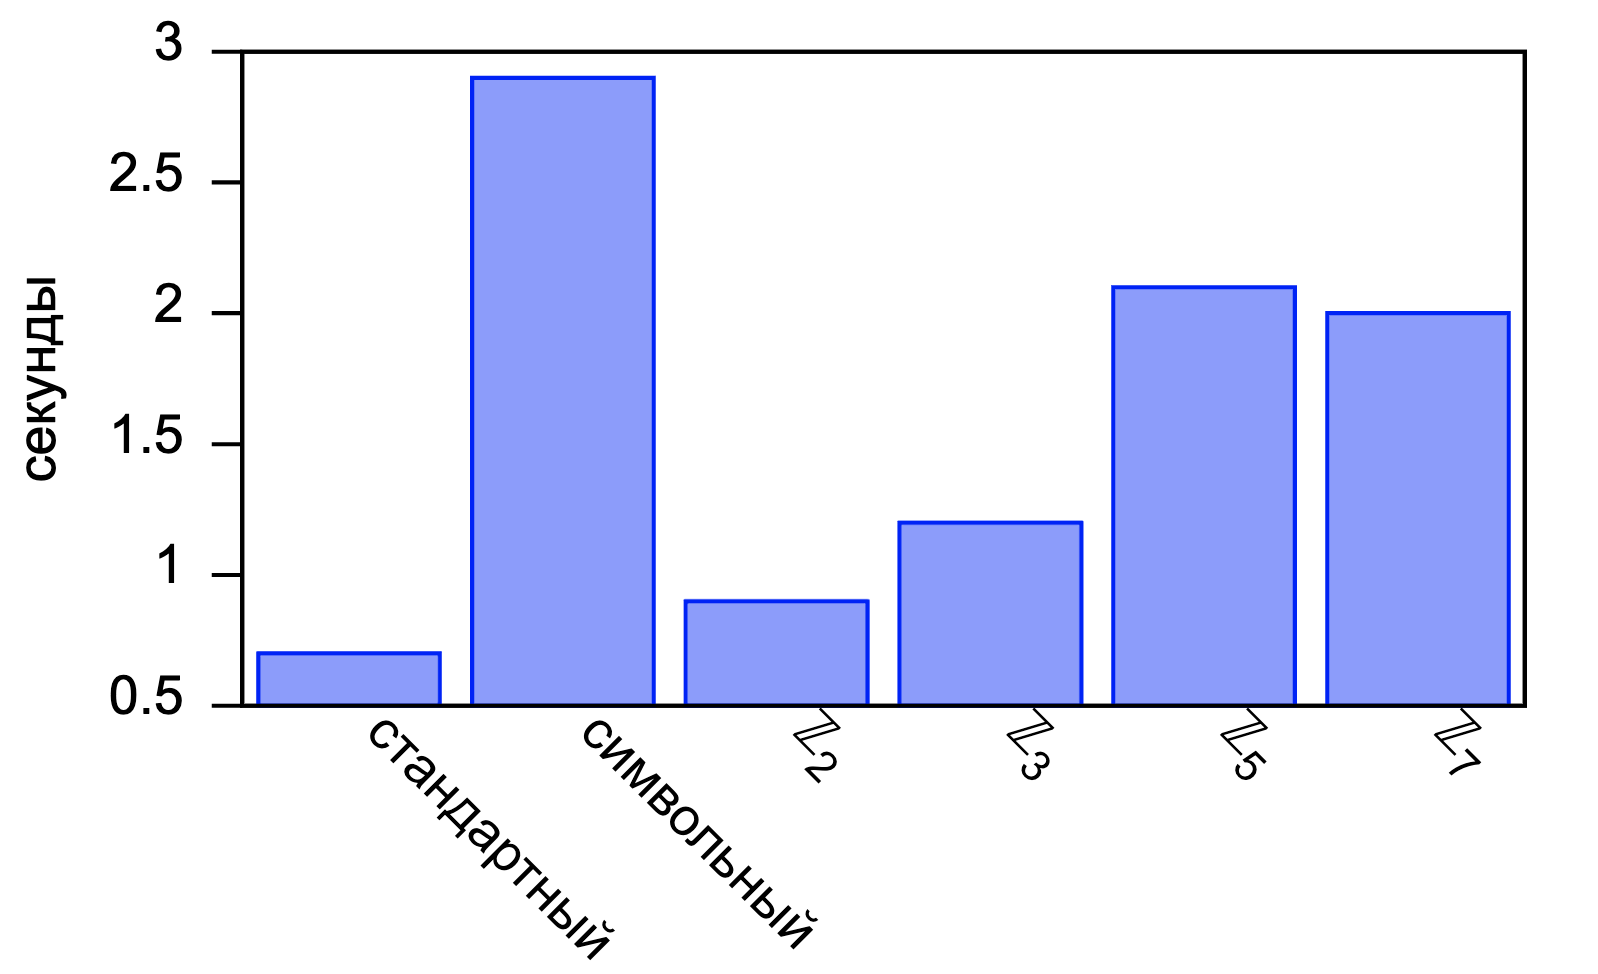
\includegraphics[width=0.85\linewidth]{../gnuplot/single/det/plot.png}}
\caption{todo}
\label{img:single:det}
\end{figure}

Как видно из результатов обычные методы работают немного быстрее, чем $p$-адические методы с числами из $\mathbb{Z}_2$ и $\mathbb{Z}_3$. Время вычисления определителя с числами из $\mathbb{Z}_5$ и $\mathbb{Z}_7$ значительно (в три раза) уступает классическим методам.


\subsubsection{Решение СЛАУ}
Для сравнения производительности классического и $p$-адического метода решения СЛАУ решим $m$ раз систему из $n$ уравнений 

$$
\boldsymbol{A}*\boldsymbol{X}=\boldsymbol{B}
$$

\noindent где $\boldsymbol{A}$ - матрица коэффициентов размером $n \times n$, $\boldsymbol{X}$ - вектор неизвестных и $\boldsymbol{B}$ - вектор правых частей.
Пусть коэффициенты матрицы $\boldsymbol{A}$ вычисляются следующим образом:

$$
a_{i,j}= 
\begin{cases} 
\abs{1-rand(n)*round\bigg(i-j\bigg)^2}, i \neq j, \\ 
10, i = j.
\end{cases}
$$,

\noindent где |rand(n)| некоторое случайное число в диапазоне от $0$ до $n$.

При этом получается симметрическая положительно определенная матрица.
Например, для $n=5$ матрица $\boldsymbol{A}$ будет иметь вид:

$$
\begin{pmatrix}
  10 & 7 & 23 & 53 & 79 \\
  0 & 10 & 8 & 11 & 80 \\
  35 & 2 & 10 & 7 & 11 \\
  17 & 3 & 7 & 10 & 1 \\
  72 & 63 & 11 & 1 & 10
\end{pmatrix}
$$

Пусть на каждом шаге решения $k=1 \dots m$ коэффициенты вектора правых частей равны номеру шага: $b_i = k$.
Чтобы контролировать правильность решения каждым программным средством будем подсчитывать сумму коэффициентов вектора $\boldsymbol{X}$ на каждом шаге решения и суммировать ее по шагам:

$$
S = \sum\limits_{k=1}^{m}\sum\limits_{i=1}^{n} x_i^{(k)}.
$$

Тестировать будем два классических метода решения уравнений - метод Гаусса и метод Крамера.

Оба метода будем тестировать при размере матрицы $n=100$ и числе повторений $m=100$ шагов. При этих параметрах должно получаться $S\approx 224,39195$.

Договоримся, что разложение (факторизацию) матрицы $\boldsymbol{A}$ будем делать на каждом шаге, т.е. каждый раз систему уравнений будем решать полностью.

Время решения будем измерять по циклу решения СЛАУ – без учета предварительной подготовки матрицы $\boldsymbol{A}$.

Разные запуски реализаций решения на ПК дают несколько разное время т.к. ОС периодически отбирает ресурсы от нашей программы для своих нужд. Из нескольких запусков будем записывать минимальное время.

Будем, для наглядности, так же сравнивать различные числа из различных полей, таких как $\mathbb{Z}_2$, $\mathbb{Z}_3$, $\mathbb{Z}_5$, $\mathbb{Z}_7$.
 
\begin{figure}[H]
\centerline{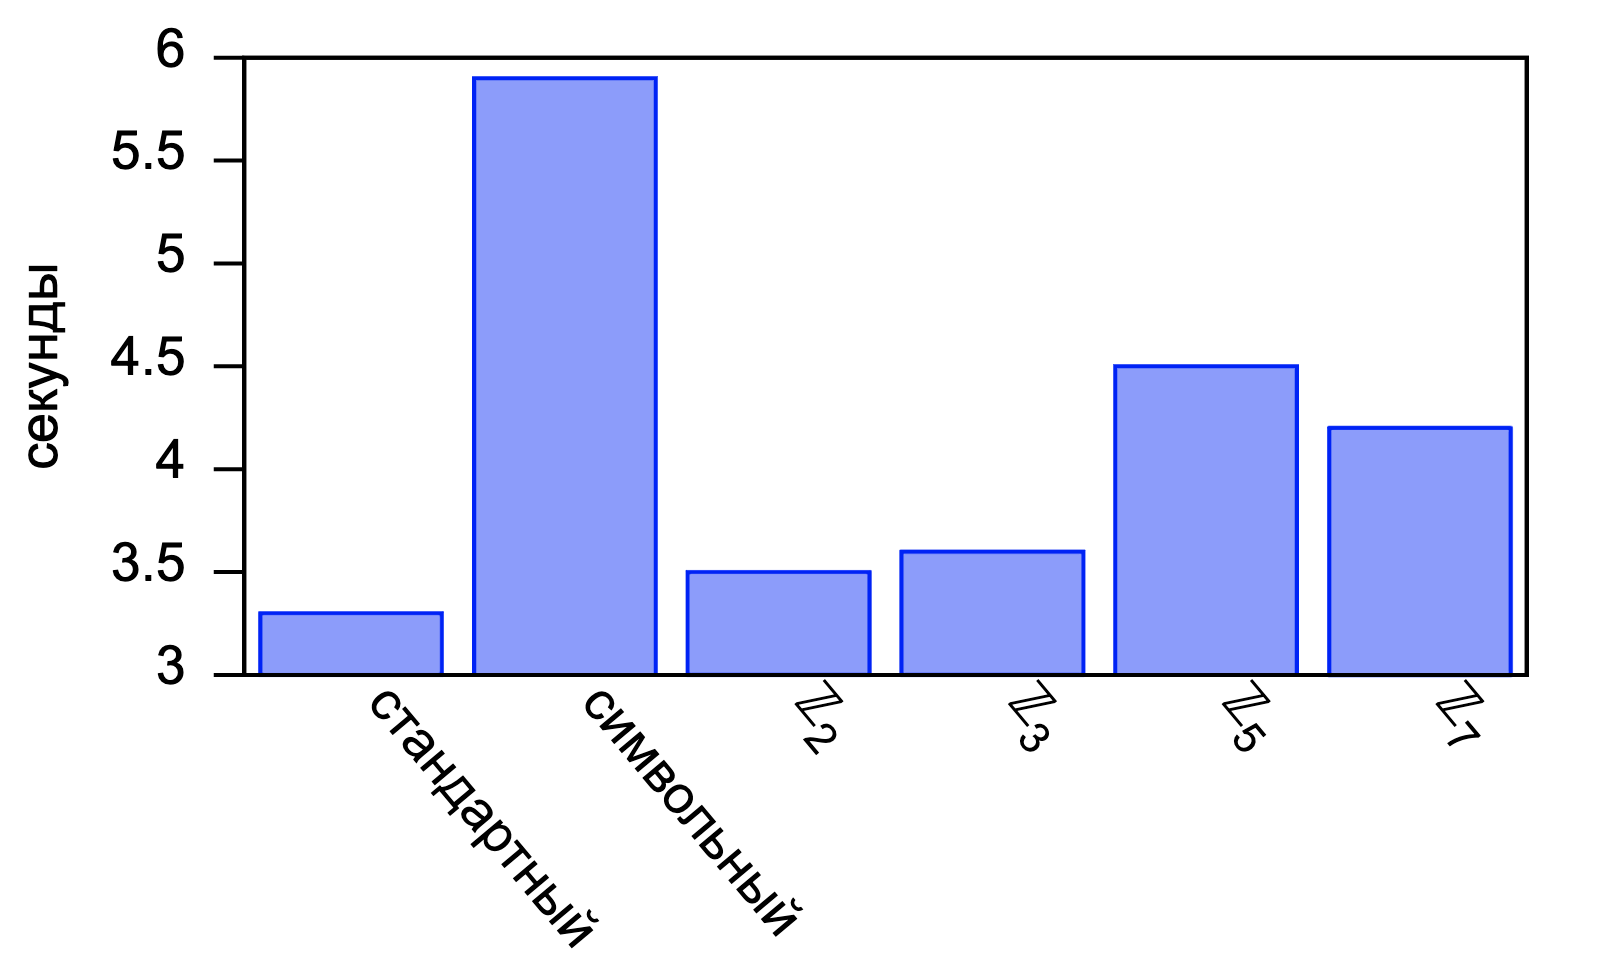
\includegraphics[width=0.85\linewidth]{../gnuplot/single/system_gauss/plot.png}}
\caption{метод Гаусса}
\label{img:single:system}
\end{figure}

\begin{figure}[H]
\centerline{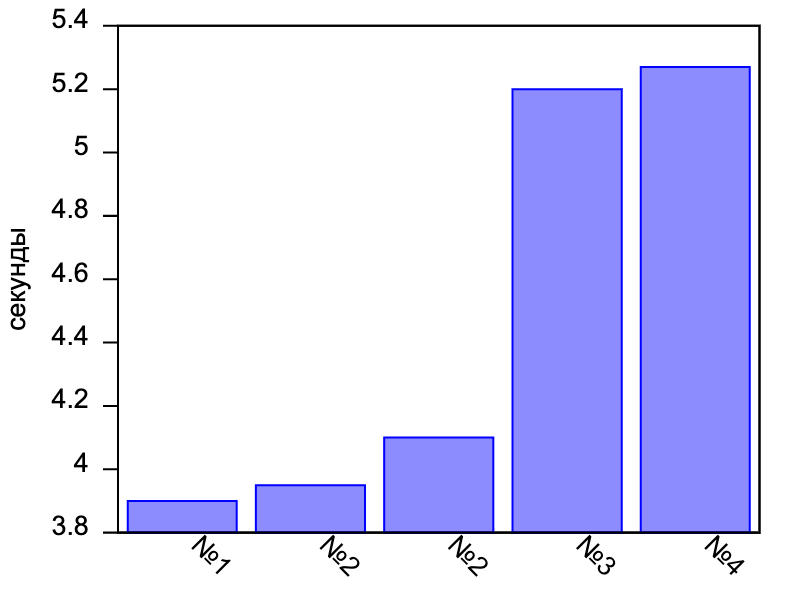
\includegraphics[width=0.85\linewidth]{../gnuplot/single/system_cramer/plot.png}}
\caption{метод Крамера}
\label{img:single:system}
\end{figure}
 
 Как видно из результатов обычные методы работают немного быстрее, чем $p$-адические методы с числами из $\mathbb{Z}_2$ и $\mathbb{Z}_3$. Время решения СЛАУ с числами из $\mathbb{Z}_5$ и $\mathbb{Z}_7$ значительно (в полтора раза) уступает классическим методам.
 
 %-------------------------------------------------------------------%
\section{Разработка многопоточной библиотеки для работы с $p$-адической арифметикой}

\subsection{Описание алгоритмов для арифметических операций}
TODO: добавить после имплементации

\subsection{Многопоточный метод решения СЛАУ}
Стандартная схема вычисления вектора $\boldsymbol{x}$ для СЛАУ $\boldsymbol{A}\cdot \boldsymbol{x} = b$ содержит представление рациональных чисел с помощью $p$-адических чисел в виде кода Гензеля и выполнении операций над данными числами. Однако, как видно из теоремы \ref{th:backward_mapping} представление чисел в виде кода Гензеля $\mathbb{H}_{p,r}$ возможно только когда ожидаемый результат будет принадлежать множеству $\mathbb{F}_{p,r}$. Это значит, что неоходимо произвести правильный выбор чисел $p$ и $r$.


Перед тем как переходить к описанию параллельного метода необходимо представить последовательный метод Гаусса.

\begin{problem}
Пусть дана матрица $\boldsymbol{A} \in \mathbb{Q}^{n \times n}$ вектор $\boldsymbol{b} \in \mathbb{Q}^{n}$. Найти вектор $\boldsymbol{x}=(x_1,\cdots,x_n) \in \mathbb{Q}^{n}$ такой, что:

\begin{equation}
\boldsymbol{A}\cdot \boldsymbol{x} = b.
\end{equation}

\end{problem}

Для начала предположим, что $\boldsymbol{A} \in \mathbb{Z}^{n \times n}$ и $\boldsymbol{b} \in \mathbb{Z}^{n}$. Используя правило Крамера мы знаем, что 

\begin{equation}\label{formula:kramer}
x_i=\frac{\Delta_i}{\Delta_i},	
\end{equation}

\noindent где $\Delta$ это определитель матрицы $A$, а $\Delta_i$ это определитель, получаемый из определителя $\Delta$ путем замены $i$-го столбца на столбец свободных членов. Известно, что если взять для любой матрицы $\mathbb{Z}^{n \times n}$ число $a$, которое будет максимальным среди остальных элементов, то оно будет удоволетворять неравенству

\begin{equation}
\mid M \mid \leq n!a^n.
\end{equation}

\noindent Из этого выражения и формулы \ref{formula:kramer} получим, что числитель и знаменатель для любого $x_i$ ограничен числом $n!a^n$, где $a$ максимальное значение матрицы $A$. Из этого ограничения можно определить число $r \in \mathbb{F}_{p,r}$ для данного простого числа $p$. Из определения достаточно того, что

\begin{equation}\label{formula:det:1}
n!a^b \leq \sqrt{\frac{p^r-1}{2}}.
\end{equation}

Принимая во внимание квадрат в левой стороне неравенства мы получаем, что 

\begin{equation}
2{(n!a^n)}^2+1\leq p^r.
\end{equation}

Неравенство в свою очередь аналогично следующему:

\begin{equation} \label{eq:matrix:r}
r \geq log_p(2{(n!a^n)}^2+1).
\end{equation}

Известно, что неравенство Адамара рассмотренное в например \cite{bib:numbers:mignotte} и \cite{bib:numbers:marcus} представляет следующее ограничение для определителя:

\begin{equation}
{\mid A \mid}^2 \leq \prod\limits_{i=1}^{n}{\bigg(\sum\limits_{j=1}^{n} a^2_{i,j} \bigg)}^{\frac{1}{2}}
\end{equation}

Из этого неравенства и неравенства \ref{formula:det:1} следует условие:

\begin{equation}
p^r \leq \sum\limits_{i=1}^{n} {\mid b_i \mid} \prod\limits_{i=1}^{n}{\bigg(\sum\limits_{j=1}^{n} a^2_{i,j} \bigg)}^{\frac{1}{2}}.
\end{equation}

Должно быть отмечено, что оба ограничения являются строгими и меньший выбор чисел $p$ и $r$ частно достаточен. В обычном случае $A \in \mathbb{Q}^{n \times n}$ и и $\boldsymbol{b} \in \mathbb{Q}^{n}$ ограничением для числителя и знаменателя для числа $x_i$ становится $n!a^{n(n+1)}$. 

\begin{thethm}
Пусть $n_1,n_2,\dots, n_k$ - натуральные попарно взаимно простые числа, а $r_1,r_2,\dots,r_k$ - некоторые целые числа, тогда существует такое целое число $M$, что оно будет решением системы сравнений:

\begin{equation}
\begin{cases} 
M \equiv r_1 \pmod {n_1}, \\
M \equiv r_2 \pmod {n_2}, \\
\dots \\
M \equiv r_k \pmod {n_k}.
\end{cases}
\end{equation}

\noindent При этом для любых двух решений $A$ и $B$ этой системы справедливо

\begin{equation}
A \equiv B \pmod {n_1,n_2,\dots,n_k},
\end{equation}

\noindent то есть решение системы сравнений существует и единственно по модулю $n_1,n_2,\dots,n_k$.
\end{thethm}


Будем описывать параллельный алгоритм для решения СЛАУ для $k$ процессов (или независимых потоков). Для начала нужно вычислить $k$ простых чисел $p_1, \dots, p_k$ случайным образом, которые удовлетворяют длинне кода $r$ так, что числа из вектора $x$ содержатся в $\mathbb{F}_{g,r}$, где $g=p_1,\dots,p_k$. 
Запустим $k$ параллельных задач. Каждая из них вычисляет образ в отношении одного простого числа в представлении рациональных элементов, т.е. $H_{p_i,r}(A)$ и $H_{p_i,r}(b)$.
После, каждый процесс запускает метод Гаусса.

\begin{algorithm}
\DontPrintSemicolon % Some LaTeX compilers require you to use \dontprintsemicolon instead

\KwIn{ $n$: степень системы \newline
       $A=(a_{i,j}) \in \mathbb{Q}^{n \times n}$: квадратная, $\dim(A)=n \times n$ \newline
       $b=(a_{1,n+1},\dots,a_{n,n+1}) \in \mathbb{Q}^{n}$: $\dim(b)=n$ \newline
       $p$: простое число }

\KwOut{$x=(x_1,\dots,x_n \in \mathbb{Q}^{n}$: решение $Ax = b$ если существует.}

\Begin {
Найти максимум $a$ среди числителей и знаменателей среди чисел входящих в состав $A$ и $b$.

Вычислить порядок числа $r$ по формуле \ref{eq:matrix:r}.

Преобразовать числа входящие из $A$ и $b$ в код Гензеля $H_{p,r}$.

l := 0\;
\For{$i \gets 1$ \textbf{to} $n$} {
  l := l + 1 \;
  \For{$j \gets 1$ \textbf{to} $n+1$} {
      Поделить $a_{i,j}$ на $a_{i,i}$.
  }
   \For{$h \gets l+1$ \textbf{to} $n$} {
      Умножить $i$-ю строку на $a_{h,l}$\;
      Вычесть полученную $i$-ю строку на $h$-ю строку системы полученную последней операцией. Это новая $h$-я строка.
  } 
}

Восстановить $H_{p,r}(x_1), \cdots, H_{p,r}(x_n)$ из полученной треугольной матрицы.
}


\caption{Алгоритм Гаусса для $p$-адической арифметики.}
\label{algo:gauss}
\end{algorithm}


Представленный алгоритм {algo:gauss} вычисляет решения $x^{(i)} \in \mathbb{H}_{p_i,r}^n$ для $i = \overline{1,k}$. После получения всех $x^{(i)}$ выполняется $k$ параллельных запусков алгоритма китайской теоремы об остатках. Будем применять параллельную версию алгоритма китайской теоремы об остатках описанную в \cite{bib:numbers:limongelli} для каждой последовательности компонентов $x_j^{(1)}, \dots, x_j^{(k)}$, получая компоненты $x_j \in \mathbb{H}_{p_1,\dots,p_k,r}$ вектора решения $x$.
Из предположений сделанных для числа $r$, полученный список результатов $\{x^{(1)},\dots,x^{(k)}\}$ может быть преобразован обратно в вектор $x \in \mathbb{F}_{g,r}^n$ с помощью китайской теоремы об остатках. Из теоремы \ref{th:hensel} известно, что если решение существует в $\mathbb{F}_{g,r}$, то оно уникальное.
После этого, результат $x$ должен быть сконвертирован из $p$-адического представление, в обычное с помощью теоремы \ref{th:backward_mapping}, применимой параллельно к каждому из компонентов. Схема параллельных вычислений представлена ниже на рисунке \ref{img:multi:gauss}.

\begin{figure}[H]
\centerline{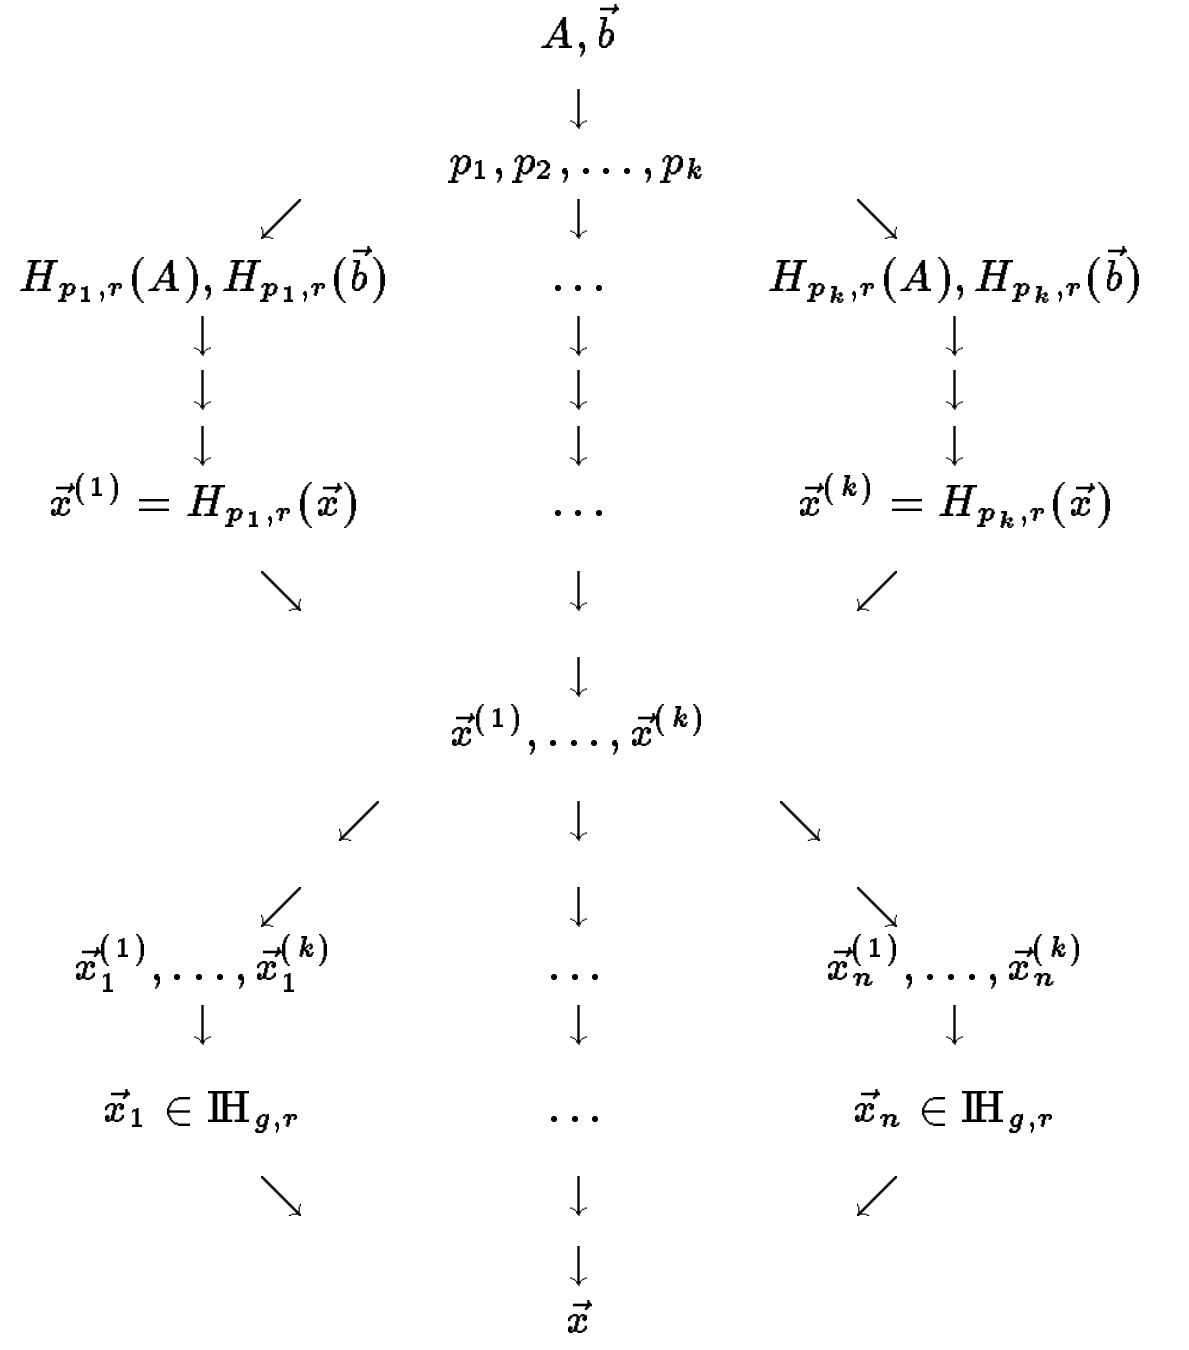
\includegraphics[width=0.7\linewidth]{images/multi/native.png}}
\caption{Схема параллельного вычисления решения СЛАУ методом Гаусса.}
\label{img:multi:gauss}
\end{figure}


В случае с матрицами больших размерностей, в разы больших, чем количество доступных процессоров, могут быть использованы стандартные методы для распараллеливания матричных операций.


\subsection{Многопоточный метод для вычисления собственных значений и собственных векторов}

Нахождение собственных значений и собственных векторов матриц - одна тех сложных вычислительных задач, с которой часто приходится сталкиваться специалисту, занимающемуся проектированием или анализом больших технических систем.

В электрических и механических системах собственные числа отвечают собственным частотам колебаний, а собственные векторы характеризуют соответствующие формы колебаний.

В теории динамических систем и связанных с ними системах линейных дифференциальных уравнений, знание собственных значений позволяет определить характер поведения системы во времени и решить вопрос об устойчивости такой системы. Оценка величин критических нагрузок при расчете строительных конструкций также основана на информации о собственных значения и собственных вектора матриц. 

Одним из методов нахождения нахождения собственных векторов и собственных значений является метод Якоби или как его еще называют метод вращений. Метод Якоби был предложен Карлом Густавом Якоби в 1846 году и представляет собой итерационный алгоритм вычисления собственных значений и собственных векторов симметричной матрицы. Метод основан на построении последовательности матриц, которые ортогонально подобны исходной матрице и имеют монотонно убывающие до нуля суммы всех внедиагональных элементов. Данный метод так же без существенных изменений метод вращений переносится на эрмитовы и косоэрмитовы матрицы. В данной работе будет рассматривать только метод, где матрица $A$ является вещественной и симметричной. Алгоритмы для случая комплексной эрмитовой матрицы можно посмотреть в \cite{bib:numbers:voevodin}.

Прежде чем переходить к описанию алгоритма и рассмотрению его особенностей связанных с применением $p$-адической арифметики необходимо ввести несколько определений.


\begin{defn}
Число $\lambda$ называется собственным значением матрицы $A$, если существует такой ненулевой вектор $x=(x_1,x_2,\cdots,x_n)$ удоволетворяющий уравнению

\begin{equation}
Ax=\lambda x
\end{equation}
	
\noindent и называемый собственным вектором матрицы $A$, отвечающим собственному значению $\lambda$.
\end{defn}


\begin{defn}
Матрицей вращения или матрицей поворота называется ортогональная матрица, которая используется для выполнения собственного ортогонального преобразования в евклидовом пространстве. При умножении любого вектора на матрицу поворота длина вектора сохраняется. Определитель матрицы поворота равен единице.
\end{defn}

Будем описывать параллельный алгоритм для нахождения собственных значений и собственных векторов матрицы $A$ для $k$ процессов (или независимых потоков). Для начала нужно вычислить $k$ простых чисел $p_1, \dots, p_k$ случайным образом, которые удовлетворяют длинне кода $r$ так, что числа из вектора $x$ содержатся в $\mathbb{F}_{g,r}$, где $g=p_1,\dots,p_k$. 
Запустим $k$ параллельных задач. Каждая из них вычисляет образ в отношении одного простого числа в представлении рациональных элементов, т.е. $H_{p_i,r}(A)$ и $H_{p_i,r}(b)$. После этого выполняется последовательный метод Якоби.

Алгоритм \ref{algo:jacoby} вычисляет значения $\lambda_i$ и $x_i$ для матрцы $A$. После получения всех собственных векторов и всех собственных чисел выполняется $k$ параллельных запусков китайской теоремы об остатках. Будем применять параллельную версию китайской теоремы об остатках описанную в \cite{bib:numbers:limongelli} для каждой последовательности компонентов $x_j^{(1)}, \dots, x_j^{(k)}$ и $\lambda_j^{(1)}, \dots, \lambda_j^{(k)}$, получая компоненты $x_j \in \mathbb{H}_{p_1,\dots,p_k,r}$ и $\lambda_j \in \mathbb{H}_{p_1,\dots,p_k,r}$

Полученный список результатов $\{x^{(1)},\dots,x^{(k)}\}$ может быть преобразован обратно в вектор $x \in \mathbb{F}_{g,r}^n$ с помощью китайской теоремы об остатках.

После этого, результа должен быть сконвертирован из $p$-адического представления, в обычное с помощью теоремы \ref{th:backward_mapping}, применимой параллельно к каждому из компонентов.

\begin{algorithm}
\DontPrintSemicolon % Some LaTeX compilers require you to use \dontprintsemicolon instead

\KwIn{ $n$: степень системы \newline
       $A=(a_{i,j}) \in \mathbb{Q}^{n \times n}$: симметричная, $\dim(A)=n \times n$ \newline
       $p$: простое число }

\KwOut{ $\lambda$: вектор содержащий все собственные значения матрицы $A$ \newline
        $x$: список содержащий все собственные вектора матрицы $A$ }

\Begin {
Найти максимум $a$ среди числителей и знаменателей среди чисел входящих в состав $A$.

Вычислить порядок числа $r$ по формуле \ref{eq:matrix:r}.

Преобразовать числа входящие из $A$ в код Гензеля $H_{p,r}$.

Инициализацировать $e, E$ и массивы $ind, changed$.

$E := I; \; state := n;$

\For{$k \gets 1$ \textbf{to} $n$} {
	$ind_k := maxind(k); \; e_k := S_{kk}; \; changed_k$ := true 
}

\While{$state \neq 0$} {
	$m := 1$
	
	%! find index (k,l) of pivot p
	\For{$k \gets 2$ \textbf{to} $n-1$} {
		\lIf{ \abs{S_{k,ind_{k}}} > \abs{S_{m,ind_{m}}} } {
			$m := k$
		}
	}
	$k := m; \; l := ind_m; \; p := S_{kl};$
	
	$c = \cos(\phi); \; s = \sin(\phi);$
	
    $y := (e_l-e_k)/2; \; d := \mid y \mid +\sqrt{p_2+y_2};$
    
    $r := \sqrt{p_2+d_2}; c := d/r; \; s := p/r; t := p_2/d;$
   	
   	\lIf{ y < 0 } {
		$s := -s; t := -t$
	}
	
	$S_kl := 0;$ 
	
	$update(k,-t); \; update(l,t)$
	
	%! rotate rows and columns k and l
	\lFor{$i \gets 1$ \textbf{to} $k-1$} {
		$rotate(i,k,i,l)$
	}
	\lFor{$i \gets k+1$ \textbf{to} $l-1$} {
		$rotate(k,i,i,l)$
	}
	\lFor{$i \gets l+1$ \textbf{to} $n$} {
		$rotate(k,i,l,i)$
	}
	%! rotate eigenvectors
	
	\lFor{$i \gets 1$ \textbf{to} $n$} {
	$$
	\begin{pmatrix}
	  E_{ik} 
	  E_{il} 
	\end{pmatrix}
	:=
	\begin{pmatrix}
	  c & -s \\
	  s & c
	\end{pmatrix}
	\cdot
	\begin{pmatrix}
	  E_{ik} 
	  E_{il} 
	\end{pmatrix}
	$$
	}
	%! rows k, l have changed, update rows indk, indl
    $ind_k := maxind(k); \; ind_l := maxind(l);$
}
}
Восстановить $H_{p,r}(x_1), \cdots, H_{p,r}(x_n)$ и $H_{p,r}(\lambda_1), \cdots, H_{\lambda,r}(\lambda_n)$.
\caption{Алгоритм Якоби для $p$-адической арифметики.}
\label{algo:jacoby}
\end{algorithm}











%-------------------------------------------------------------------%
\section{Сравнение производительности классических и $p$-адических методов на примере прикладных задач}


Все тесты в этом параграфе будут производятся на компьютере с процессором Intel Core i5-7360U и 16 Гб оперативной памяти. Для тестов будем использовать 4 параллельных потока.


\subsection{Решение СЛАУ}
Подход к тестированию вычисления решения СЛАУ будет производится тем же методом, что и в случае однопоточной программы. Сравнение будет производить с символьным методом решения СЛАУ из пакета |scipy|, с методом для решения СЛАУ из пакета |numpy|, с однопоточным и многопоточным $p$-адическим методом Гаусса. В случае с $p$-адическими методами будем использовать числа из $\mathbb{Z}_2$, $\mathbb{Z}_3$, $\mathbb{Z}_5$, $\mathbb{Z}_7$. 


\begin{figure}[H]
\centerline{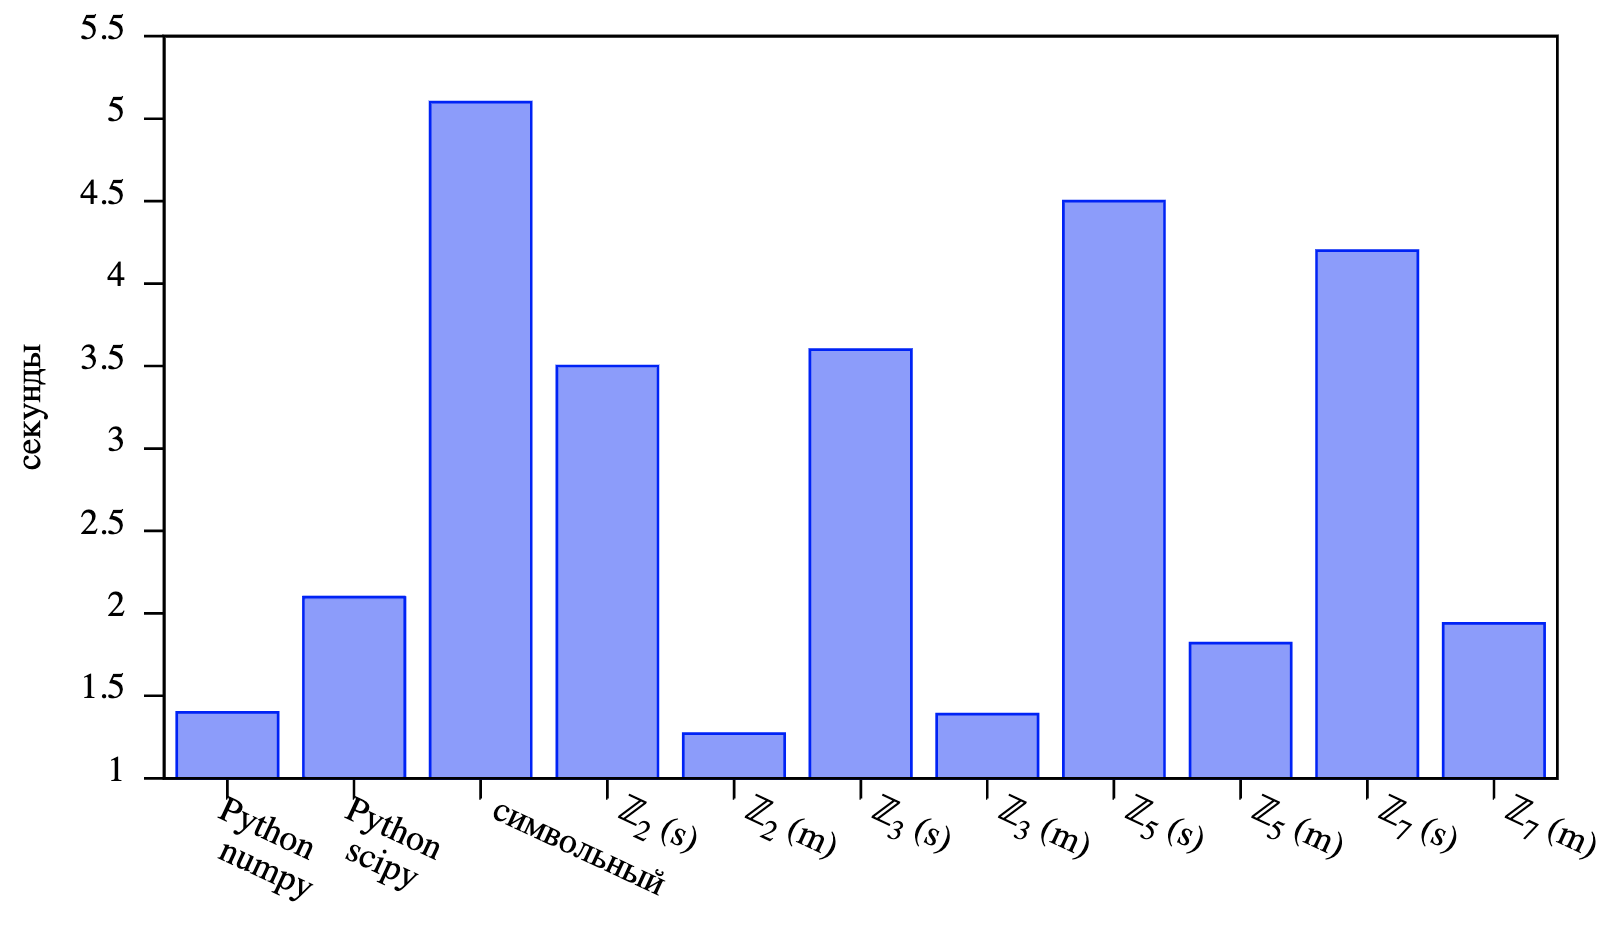
\includegraphics[width=0.85\linewidth]{../gnuplot/comp/gauss/plot.png}}
\caption{todo}
%\label{img:single:det}
\end{figure}

\subsection{TODO}
%{Вычисление собственных значений и собственных векторов
Сравнение вычисления собственных значений и собственных векторов симметричной матрицы $A$ будем производить с помощью итерационного метода Якоби называемого методом вращений, который основан на приведении матрицы $A$ к диагональному виду.

Идея метода Якоби состоит в том, чтобы обнулять недиагональные элементы вращениями до тех пор, пока они все не обнулятся и получится диагональная матрица. После каждого вращения сумма квадратов внедиагональных элементов уменьшается, что приводит к сходимости процесса диагональности. 


\begin{figure}[H]
\centerline{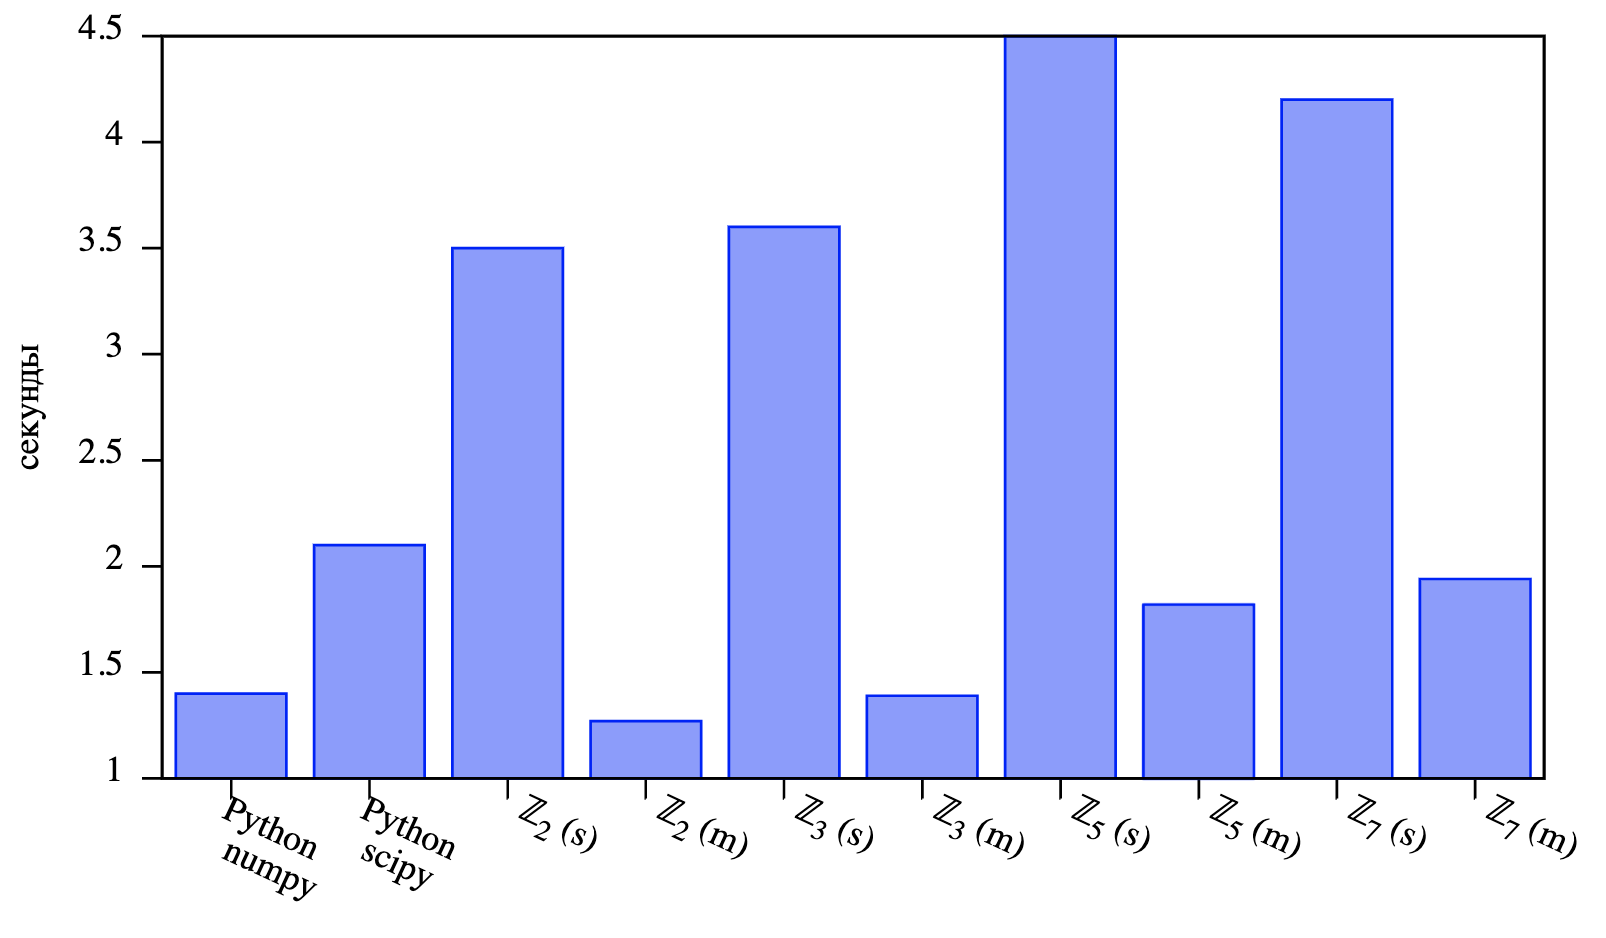
\includegraphics[width=0.85\linewidth]{../gnuplot/comp/jacoby/plot.png}}
\caption{todo}
%\label{img:single:det}
\end{figure}

\subsection{Решение ОДУ}
Для сравнения методов возьмем дифференциальное уравнение падающей сферы:

\begin{equation}
\begin{aligned}
\dfrac{\partial z}{ \partial t} = v \\
\dfrac{\partial v}{ \partial t} = g - \alpha v^2
\end{aligned}
\end{equation}

\noindent где

\begin{equation}
\begin{aligned}
\alpha = \frac{3\rho_f}{4\rho_k d}C_d
\end{aligned}
\end{equation}

\noindent аналитическое решение данного уравнения при $z(0)=0$ и $v(0)=0$ будет следующее:

\begin{equation}
\begin{aligned}
z(t)=\frac{ln(cosh(\sqrt{\alpha g} \cdot t)}{\alpha} \\
v(t)=\sqrt{\frac{g}{\alpha}} \cdot tanh{\sqrt{\alpha g} \cdot t)}
\end{aligned}
\end{equation}

Конечная скорость $v_t$ находится из уравнения $\frac{\partial v}{ \partial t}$ и равна $v_t=\sqrt{\frac{g}{\alpha}}$.

В качестве физических параметров для эксперимента будем использовать параметры стандартного мяча для гольфа:

\begin{threeparttable}
\begin{longtable}[H]{lp{0.7\linewidth}}
{$d$} -- диаметр шара & 41 [мм] \\
{$\rho_k$} -- плотность сферы & 1275 [кг/м\textsuperscript{3}] \\
{$\rho_f$} -- плотность жидкости & 1.22 [кг/м\textsuperscript{3}] \\
{$C_d$} -- коэффициент трения & 0.4 
\end{longtable} 
\end{threeparttable}


При этих параметрах $\alpha$=$7 \cdot 10^{-3}$, а конечная скорость становится равной $v_t=\sqrt{\frac{g}{\alpha}}=37.44$.


Для сравнения методов будет использоваться схема метода Рунге-Кутты 4-го порядка:

\begin{equation}%\label{eq:task:2}
\begin{aligned}
k_1 = f(x_n, y_n) \\
k_2 = f(x_n+\frac{h}{2}, y_n+\frac{h}{2}k_1) \\
k_3 = f(x_n+\frac{h}{2}, y_n+\frac{h}{2}k_2) \\ 
k_4 = f(x_n+h, y_n+hk_3) \\
y_{n+1}=y_n+\frac{h}{6}(k_1+2k_2+2k3+k_4)
\end{aligned}
\end{equation}


\noindent И схема метода Эйлера:

\begin{equation}%\label{eq:task:2}
\begin{aligned}
y_{n+1}=y_n+h \cdot f(x_n, y_n)
\end{aligned}
\end{equation}

Разные запуски реализаций решения на ПК дают несколько разное время т.к. ОС периодически отбирает ресурсы от нашей программы для своих нужд. Запускать тесты для большей точности вычислений будем $10$ раз. Из нескольких запусков будем записывать минимальное время.

Для наглядности будем так же сравнивать различные числа из различных полей, таких как $\mathbb{Z}_2$, $\mathbb{Z}_3$, $\mathbb{Z}_5$ и $\mathbb{Z}_7$.


\begin{figure}[H]
\centerline{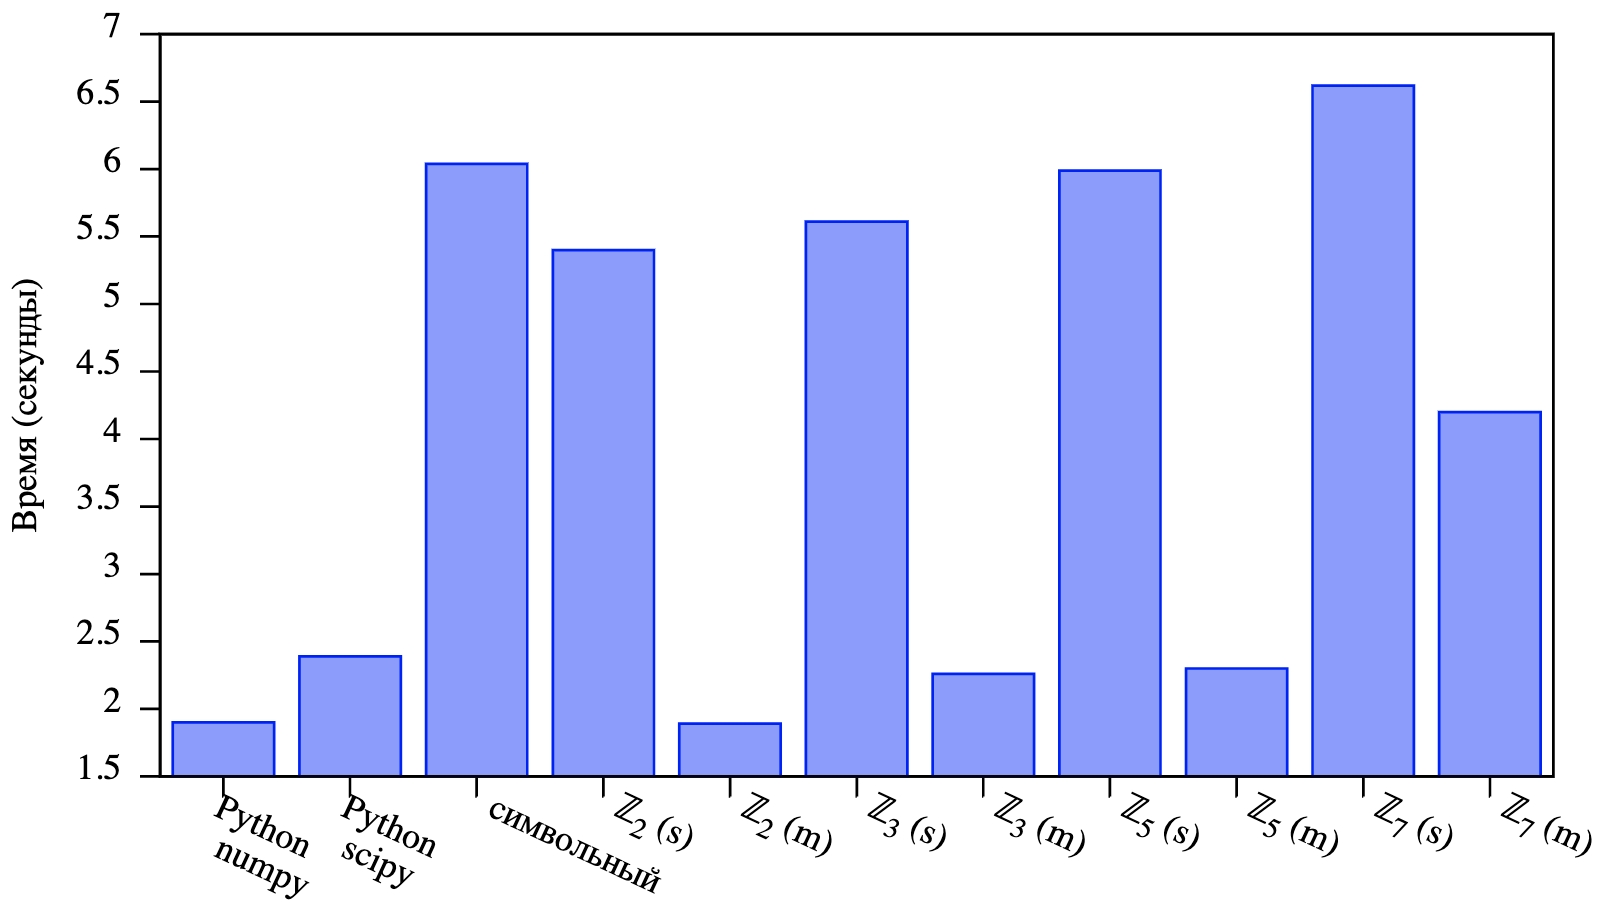
\includegraphics[width=0.85\linewidth]{../gnuplot/comp/euler/plot.png}}
\caption{todo}
%\label{img:single:det}
\end{figure}

\begin{figure}[H]
\centerline{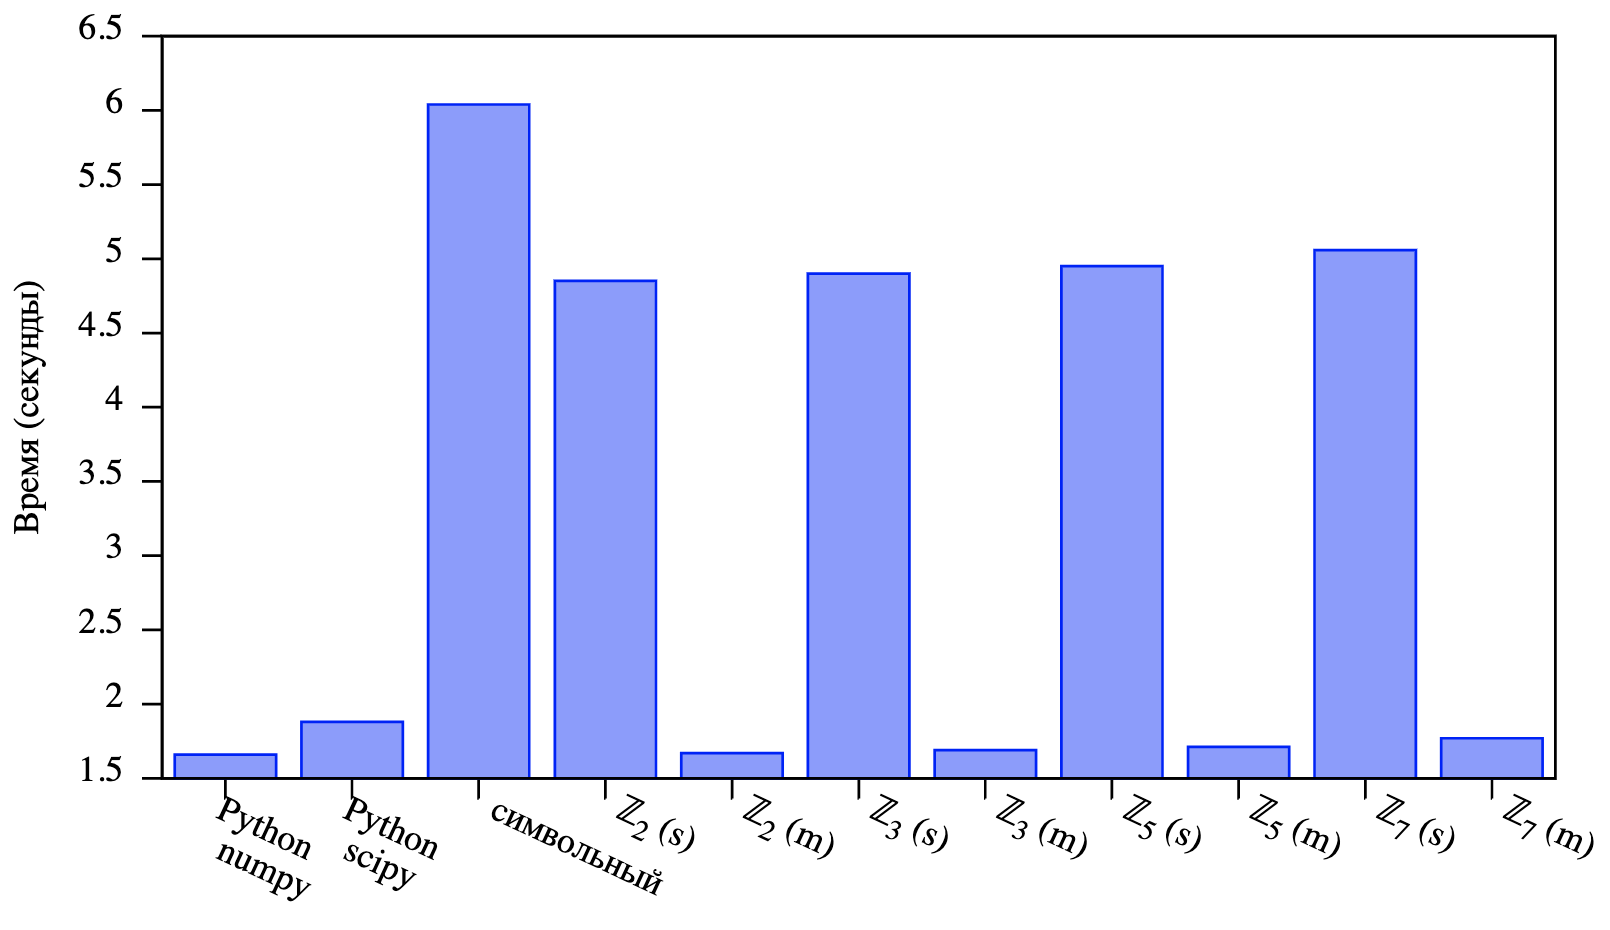
\includegraphics[width=0.85\linewidth]{../gnuplot/comp/rk/plot.png}}
\caption{todo}
%\label{img:single:det}
\end{figure}

\begin{figure}[H]
\centerline{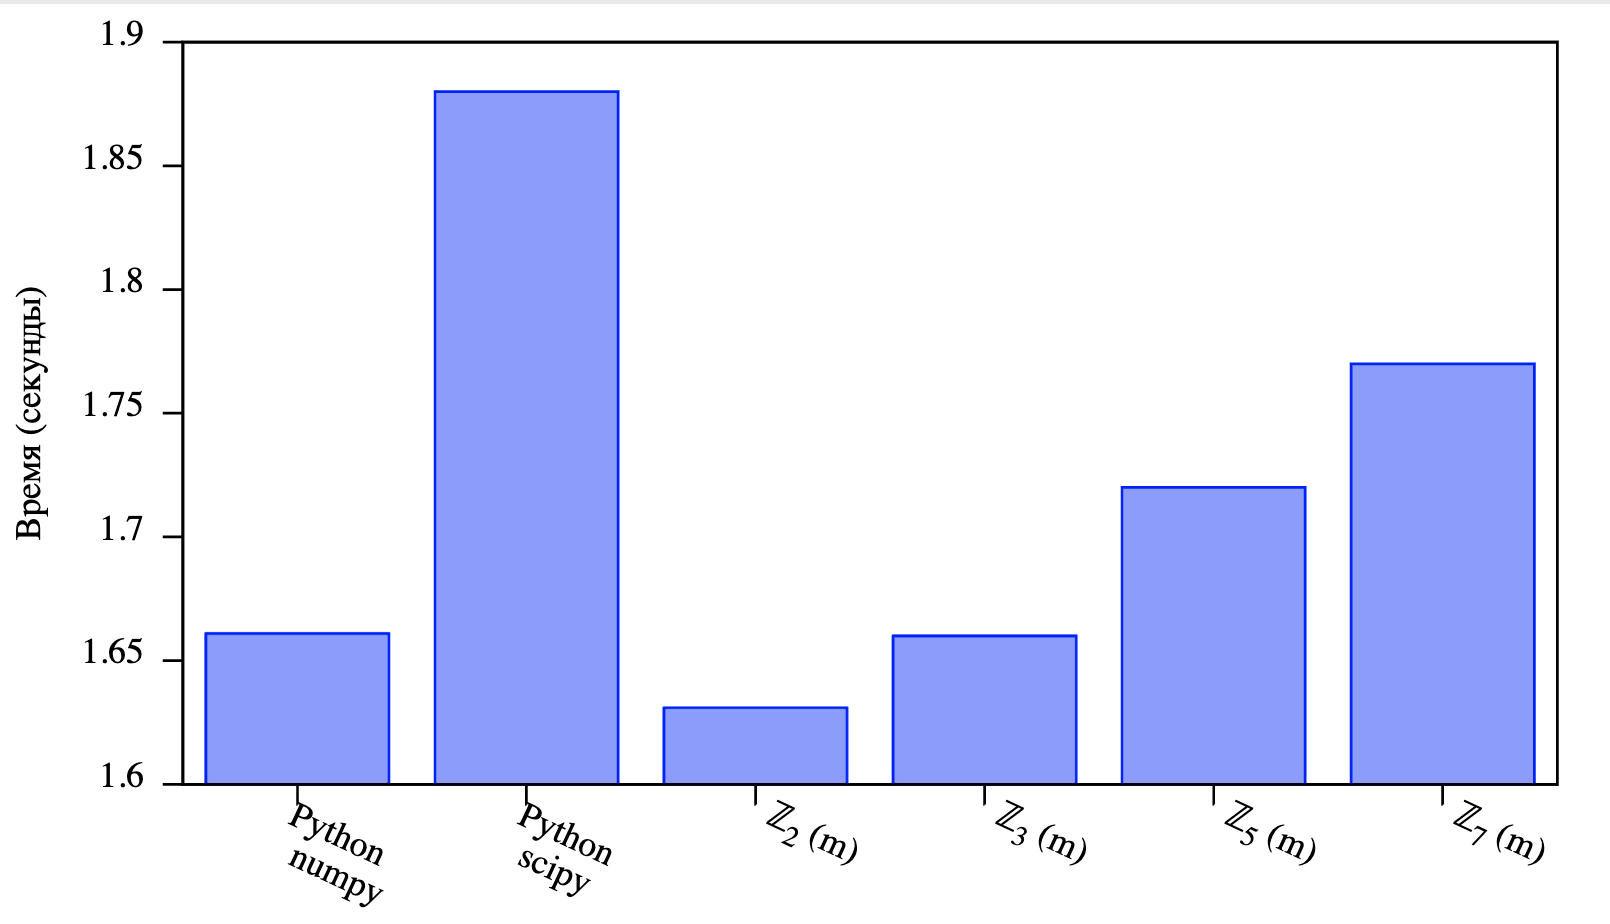
\includegraphics[width=0.85\linewidth]{../gnuplot/comp/rk/multi.png}}
\caption{todo}
%\label{img:single:det}
\end{figure}


\subsection{Вычисление $e^{Ax}$}

todo для чего оно нужно
Эффективность некоторых алгоритмов вычислений экспоненты
матрицы сильно зависит от вида матрицы. Существенную роль в некоторых подходах играют собственные значения и собственные векторы
матрицы, даже если они не вовлечены в конкретный алгоритм.


Для вычисления $e^{At}$ будем использовать полиномиальный метод, но перед этим необходимо ввести ряд определний.

\begin{defn}
Фробениусовой нормальной формой линейного оператора $А$ называется каноническая форма его матрицы, соответствующая минимальному разложению линейного пространства в прямую сумму инвариантных относительно $А$ подпространств, которые могут быть получены как линейная оболочка некоторого вектора и его образов под действием А. Она будет блочно-диагональной матрицей, состоящей из фробениусовых клеток вида

\begin{equation}
\begin{pmatrix}
0&0&\cdots&0&-a_0\\
1&0&\cdots&0&-a_1\\
0&1&\cdots&0&-a_2\\
\vdots&\vdots&\ddots&\vdots&\vdots\\
0&0&\cdots&1&-a_{n-1}
\end{pmatrix}
\end{equation}

\end{defn}

\begin{defn}
Матрица Хессенберга - разновидность квадратных матриц, обобщающая треугольные матрицы. Верхняя матрица Хессенберга — это квадратная матрица ${\displaystyle H}$, у которой все элементы лежащие ниже первой поддиагонали равны нулю, то есть 

\begin{equation}
h_{ij}=0 \; \forall i \textgreater j+1.	
\end{equation}

\noindent Аналогично определяется нижняя матрица Хессенберга, как квадратная матрица, при транспонировании которой получается верхняя матрица Хессенберга.
\end{defn}


Для вычисления $e^{At}$ необходимо сначала привести матрицу $A$ к нижней матрице Хессенберга $H$ и получить трансформированную матрицу $T$ такую, что:

\begin{equation}
T^{-1}AT=H.
\end{equation} 

Далее необходимо привести нижнюю матрицу Хессенберга к Фробениусовой нормальной форме с помощью формулы Уилкинсона,

\begin{equation}
C^{-1}WC=F.
\end{equation}

Теперь необходимо сформировать диагональную матрицы $D$ которая должна преобразовать матрицу $F$ так, чтобы субдиагональ состояла из единиц,

\begin{equation}
D^{-1}FD=G.
\end{equation}

После этих операций получается Фробениусова каноничная форма для матрицы $G$, невырожденная матрица $W$ и обратная матрица $W^{-1}$ для которой справедливо, что:

\begin{equation}
W^{-1}=D^{-1}C^{-1}T^{-1}, \; W=TCD.
\end{equation}
 
В большинстве случаев, $G$ будет иметь следующую структуру:

\begin{equation}G=
\begin{pmatrix}
0 & & \cdots & & c_0\\
1 & 0 & \cdots & & c_1\\
& \ddots & \ddots & & \vdots \\
& & 1 & 0 & c_{n-2} \\
& & & 1 & c_{n-1}
\end{pmatrix}
\end{equation}
 
\noindent В соответсвии и с теоремой Гамильтона-Кэли \cite{bib:algebra:roitenberg} получается, что:

\begin{equation}
A^n=c_0I+c_1A+\cdots+c_{n-1}A^{n-1}.
\end{equation}

Из предыдущего выражения следует, что любая степень $A$ может быть выражена в терминах $I, A, \cdots, A^{n-1}$:

\begin{equation}
A^k=\sum\limits_{j=0}^{n-1} \beta_{kj}A^j.
\end{equation}


Теперь вычисление $e^{At}$ может быть реализовано следующим образом:


\begin{equation}
e^{tA}=\sum\limits_{k=0}^{\infty} \frac{t^kA^k}{k!}=\sum\limits_{k=0}^{\infty} \frac{t^k}{k!} \cdot \sum\limits_{j=0}^{n-1} \beta_{kj} A^j = \sum\limits_{j=0}^{n-1} \cdot \bigg(\sum\limits_{k=0}^{\infty} \beta_{kj} \frac{t^k}{k!} \bigg) A^j = \sum\limits_{j=0}^{n-1} \alpha_{j}(t)A^j
\end{equation}

\noindent где $\alpha_{j}(t)$ и $\beta_{kj}$ вычисляются как:

\begin{equation}
\alpha_{j}(t)=\sum \beta_{kj} \frac{t^k}{k!},
\end{equation}

\begin{equation}
\beta_{kj} = \begin{cases} 
\delta_{kj} & (k \textless n) \\
c_j & (k = n) \\
c_0 \beta_{k-1,n-1} & (k \textgreater n, j=0) \\
c_j \beta_{k-1,n-1}+\beta_{k-1,j-1} & (k \textgreater n, j \textgreater 0)
\end{cases}.
\end{equation}



\conclusion
В представленной магистерской работе были получены, ...
Реализована возможность ...
В качестве примера были произведены расчеты на различных ...

\bibliographystyle{biblio/ugost}
\bibliography{biblio/biblio}

\appendix

\section{Исходный код библиотеки для работы с $p$-адической арифметикой}
todo

\section{Вспомогательные функции для метода Якоби}
\begin{algorithm}
\DontPrintSemicolon % Some LaTeX compilers require you to use \dontprintsemicolon instead
\KwIn{ $k$ }
\Begin {
	$m$ := $k+1$
	\For{$i \gets k+2$ \textbf{to} $n$} {
		\If{ \abs{S_{ki}} > \abs{S_{km}} } {
			$m := i$ 
		}
	}
	\Return m
}
\caption{функция $maxind$}
\end{algorithm}

\begin{algorithm}
\DontPrintSemicolon % Some LaTeX compilers require you to use \dontprintsemicolon instead
\KwIn{ $k, l, i, j$ }
\Begin {
$$
\begin{pmatrix}
  S_{kl} 
  S_{ij} 
\end{pmatrix}
:=
\begin{pmatrix}
  c & -s \\
  s & c
\end{pmatrix}
\cdot
\begin{pmatrix}
  S_{kl} 
  S_{ij} 
\end{pmatrix}
$$
}
\caption{процедура $rotate$}
\end{algorithm}

\begin{algorithm}
\DontPrintSemicolon % Some LaTeX compilers require you to use \dontprintsemicolon instead
\KwIn{ $k, t$ }
\Begin {
$y := e_k$ 
$e_k := y+t$
\If{$changed_k$ И ($y=e_k$)} {
	$changed_k$ := false
	state := state-1
}
\If {не $changed_k$) И ($y \neq e_k$)} {
	$changed_k$ := true
	state := state+1
}
}
\caption{функция $update$}
\end{algorithm}


\end{document}